\chapter{Information-theoretic evaluation of predicted ontological annotations}
\label{ch:rumi}

%\begin{center}
%\[ pub placeholder \]
%\[ pub placeholder \]
%
%\end{center}


%%%%%%%%%%%%%%%%%%%%%%
%%%%%%%%%%%%%%%%%%%%%%


Ontological representations have been widely used in biomedical sciences to standardize knowledge representation and exchange \citep{Robinson2011}. Modern ontologies are typically viewed as graphs in which vertices represent terms or concepts in the domain of interest and edges represent relational ties between terms (e.g. is-a, part-of). While, in theory, there are no restrictions on the types of graphs used to implement ontologies, hierarchical organizations, such as trees or directed acyclic graphs, have been frequently used in the systematization of biological experiments, organismal phenotypes, or structural and functional descriptions of biological macromolecules.

In molecular biology, one of the most frequently used ontologies is the Gene Ontology \citep{Ashburner2000}, which standardizes the functional annotation of genes and gene products. The development of the Gene Ontology (GO) was based on the premise that the genomes of all living organisms are composed of genes whose products perform functions derived from a finite molecular repertoire. In addition to knowledge representation, GO has also facilitated large-scale analyses and automated annotation of gene product function \citep{Radivojac2013}. As the rate of accumulation of uncharacterized sequences far outpaces the rate at which biological experiments can be carried out to characterize those sequences, computational function prediction has become increasingly useful for the global characterization of genomes and proteomes as well as for guiding biological experiments via prioritization  \citep{Sharan2007,Rentzsch2009}.

The growing importance of tools for the prediction of GO annotations, especially for proteins, presents the problem of how to accurately evaluate such tools. Because terms can automatically be associated with their ancestors in the GO graph, the task of an evaluation procedure can be framed as comparing the predicted graph with the graph represented by the true, experimentally verified annotations. It should be explicitly noted that the structure of the ontology introduces dependence between terms, dependencies that must be appropriately considered when comparing two graphs. This is obviously true for terms that share an ancestor/descendant relationship, but also for terms that are not related through direct ancestry.  For example, although the terms ``H3 histone acetyltransferase activity" and ''H4 histone acetyltransferase activity" do not share a ancestor/descendant relationship and describe different behaviors of histone acetyltransferases, they nonetheless are not independent. 

Protein function is also complex and context dependent. A single biological experiment rarely results in complete characterization of a protein's function. Furthermore, annotations might not always be meaningful; a point that is particularly evident in cases where only high-throughput experiments are used for functional characterization, leading to shallow annotation graphs. These types of annotations pose a problem in evaluation as the ground truth is incomplete and noisy. 

Furthermore, different computational models produce different outputs that must be accounted for. Some models simply assign binary yes-or-no values to terms; while others might assign a different score to potentially each node in the ontology, with an expectation that a good decision threshold would be applied to provide useful annotations.
Finally, a complicating factor is posed by the fact that GO, as most current ontologies, is generally unfinished and contains a range of specificities of functional descriptions at the same depth of the ontology \citep{alterovitz2010}.

There are two important factors related to the development of evaluation metrics. First, because both the experimental and predicted annotation of genes can be represented as subgraphs of the generally much larger GO graph, it is unlikely that a given computational method will provide an exact prediction of the experimental annotation. It is therefore necessary to develop metrics that facilitate calculating degrees of similarity between pairs of graphs and appropriately address dependency between nodes. Ideally, such a measure of similarity would be able to characterize both the level of correct prediction of the true (albeit incomplete) annotation but also the level of misannotation. The second important factor related to the evaluation metric is its interpretability. Characterizing the predictor's performance should be meaningful to a downstream user. Ideally, an evaluation metric would have a simple probabilistic interpretation. 

In this chapter, we develop an information-theoretic framework for evaluating the prediction accuracy of computer-generated ontological annotations. We first use the structure of the ontology to probabilistically model, via a Bayesian network, the prior distribution of protein experimental annotation. We then apply our metric to three protein function prediction algorithms selected to highlight the limitations of typically-considered evaluation metrics. We show that our metrics provide added value to the current analyses of the strengths and weaknesses of computational tools. Finally, we argue that our framework is probabilistically well founded and show that it can also be used to augment already existing evaluation metrics.

%%%%%%%%%%%%%%%%%%%%%%
%%%%%%%%%%%%%%%%%%%%%%
 

\section{Background}
The issue of performance evaluation is closely related to the problems of measuring similarity between pairs of graphs or sets. First, we note that a protein's annotation (experimental or predicted) is a graph containing a subset of nodes in the ontology together with edges connecting them. We use the term \emph{leaf node} to describe a node that has no descendants in the annotation graph, although it is allowed to have descendants in the ontology. A set of leaf terms completely describes the annotation graph. %In the literature, such nodes are often referred to simply as terms with an assumption that all of their ancestors are automatically included in the annotation of the protein.


We roughly group both graph similarity and performance evaluation metrics into topological and probabilistic categories, and note that a particular metric may combine aspects from both. More elaborate distinctions are provided by \cite{Pesquita2009} and \cite{Guzzi2012}. Topological metrics rely on the structure of the ontology to perform evaluation and typically employ metrics that operate on sets of nodes and/or edges. A number of topological measures have been utilized, including the Jaccard and cosine similarity coefficients (the cosine function maps the binary term designations into a vector space), the shortest path-based distances \citep{Rada1989}, etc. In the context of classifier performance analysis, two common 2D metrics are the precision/recall curve and the Receiver Operating Characteristic (ROC) curve. Both curves are constructed based on the overlap in either edges or nodes between true and predicted terms and have been widely used to evaluate the performance of tools for the inference of GO annotations. They can also be used to provide a single statistic to rank classifiers through the maximum F-measure in the case of precision/recall curve or the area under the ROC curve. The area under the ROC curve has a limitation arising from the fact that the ontology is relatively large, but that the number of terms associated with a typical protein is relatively small. In practice, this results in specificities close to one regardless of the prediction, as long as the number of predicted terms is relatively small.

Although these statistics provide good feedback regarding multiple aspects of a predictor's performance, they do not always address node dependency or the problem of unequal specificity of functional annotations found at the same depth of the graph. Coupled with a large bias in the distribution of terms among proteins, prediction methods that simply learn the prior distribution of terms in the ontology could appear to have better performance than they actually do.

The second class of similarity/performance measures are probabilistic or information-theoretic metrics. Such measures assume an underlying probabilistic model over the ontology and use a database of proteins to learn the model. Similarity is then assessed by measuring the information content of the shared terms in the ontology but can also take into account the information content of the individual annotations. Unlike with topological measures where updates to the ontology  affect similarity between objects, information theoretic measures are also affected by changes in the underlying probabilistic model even if the structure of the ontology remains the same.

Probabilistic metrics closely follow and extend the methodology laid out by \cite{Resnik1995}, which is based on the notion of information content between a pair of individual terms. These measures overcome biases related to the structure of the ontology; however, they have several drawbacks of their own. One that is especially important in the context of analyzing the performance of a predictor is that they only report a single statistic, namely the similarity or distance between two terms or sets of terms. This ignores the tradeoff between precision and recall that any predictor has to make. In the case of Resnik's metric, a prediction by any descendant of the true term will be scored as if it is an exact prediction. Similarly, a shallow prediction will be scored the same as a prediction that deviates from the true path at the same point, regardless of how deep the erroneous prediction might be. Although some of these weaknesses have been corrected in subsequent work \citep{Jiang1997,Lin1998,Schlicker2006}, there remains the issue that the available probabilistic measures of semantic similarity resort to ad hoc solutions to address the common situation where proteins are annotated by graphs that contain multiple leaf terms \citep{Clark2011}. Various approaches have been taken, including averaging between all pairs of leaf terms \citep{Lord2003}, finding the maximum among all pairs \citep{Resnik1999}, or finding the best-match average, but each such solution lacks strong justification in general. For example, all-pair averaging leads to anomalies where the exact prediction of an annotation containing a single leaf term $u$ would be scored higher than the exact prediction of an annotation containing two distinct leaf terms $u$ and $v$ of equal information content, when it is more natural to think that the latter prediction should be scored higher. Finally, all semantic similarity metrics that incorporate some form of pairwise matching between leaf terms tacitly assume that the objects to be compared are annotated by similar numbers of leaf terms. As such, they could produce undesirable solutions when applied to a wide range of prediction algorithms such as those outputting a very large number of predicted terms.


%%%%%%%%%%%%%%%%%%%%%%
%%%%%%%%%%%%%%%%%%%%%%


\section{Protein function prediction scenarios}

In protein function prediction, there are two scenarios in which a computational model can be constructed \citep{Radivojac2013}: (i) given a new protein, the task of a classifier is to find all functional terms that the protein is associated with (``what is the function of this protein?"); and (ii) given a functional term, the task of a classifier is to find all proteins associated with this term (``what are the proteins associated with this function?"). Undoubtably, the two prediction scenarios are related because a perfect predictor of protein function would solve both questions at the same time. However, imperfect predictors may address one question better than the other. For example, a classifier built to address the first question is expected to be accurate in predicting all (or many) functional terms and that prediction scores over all functional terms are comparable. On the other hand, a predictor developed to consider only one functional term at a time need not consider any other term. Such models can perform well even if they just rank all test proteins. In addition to these differences, the two types of models are evaluated in different ways (yet they use the same terminology).

Models that are concerned with predicting function on a previously unseen protein (scenario 1, above) need to devise evaluation metrics to estimate the expected accuracy of a predicted consistent graph $P$ when the experimental (true) annotation of the protein is graph $T$. Alternatively, the models that are concerned with ranking the proteins according to their likelihood to be associated with a particular functional term $v$ (scenario 2, above) need to be evaluated based on the expectation that a particular protein is associated with a functional term $v$. Here, the models are usually evaluated for each functional term $v$, one at a time. Evaluation metrics corresponding to the former problem are significantly more challenging than the metrics corresponding to the latter problem. In the latter case, one can simply consider a particular decision threshold for predicting whether a protein is associated with function $v$ and then calculate the fraction of positive predictions that are correct (precision) as well as the fraction of proteins known to be associated with functional term $v$ that have been retrieved (recall). Such evaluation has been discussed by \citet{Sharan2007}, among others. Calculating precision and recall for the former scenario is the topic of our study.

%%%%%%%%%%%%%%%%%%%%%%
%%%%%%%%%%%%%%%%%%%%%%
\section{Methods} 
\label{sec:rumiMethods}
Our objective here is to introduce information-theoretic metrics for evaluating classification performance in protein function prediction. In this learning scenario, the input space $\mathcal{X}$ represents proteins whereas the output space $\mathcal{Y}$ contains directed acyclic graphs describing protein function according to the Gene Ontology (GO). 

Because of the hierarchical nature of GO, both experimental and computational annotations need to satisfy the \emph{consistency requirements}:

\begin{enumerate}[label=\roman*.,font=\itshape]
\item

If vertex (term) $v$ from the ontology is true, then all of its ancestors must also be true.

\item
If vertex (term) $v$ from the ontology is false, then all of its descendants must also be false.

\end{enumerate}
By enforcing these requirements we frame the task of a classifier as assigning the best consistent subgraph of the ontology to each new protein and output a prediction score for this subgraph and/or each predicted term. 

We simplify the exposition by referring to such graphs as prediction or annotation graphs. In addition, we frequently treat consistent graphs as sets of nodes or functional terms and use set operations to manipulate them. %Finally, because we use Gene Ontology for describing protein function, we shall alternatively refer to the GO graph as an ontology. 

We now proceed to provide a definition for the information content of a (consistent) subgraph in the ontology. Then, using this definition, we derive information-theoretic performance evaluation metrics for comparing pairs of graphs.

%%%%%%%%%%%%%%%%%%%%%%
%%%%%%%%%%%%%%%%%%%%%%
\subsection{Calculating the joint probability of a graph}
%%%%%%%%%%%%%%%%%%%%%%
%%%%%%%%%%%%%%%%%%%%%%


Let each term in the ontology be a binary random variable and consider a fixed but unknown probability distribution over $\mathcal{X}$ and $\mathcal{Y}$ according to which the quality of a prediction process will be evaluated. We shall assume that the prior distribution of a target can be factorized according to the structure of the ontology, i.e. we assume a Bayesian network as the underlying data generating process for the target variable. According to this assumption, each term is independent of its ancestors given its parents and, thus, the full joint probability can be factorized as a product of individual terms obtained from the set of conditional probability tables associated with each term \citep{Koller2009}, 

\begin{equation}
\Pr(\mathbf{V})=\underset{v\in \mathbf{V} }{\prod}\Pr(v|\mathcal{P}(v)),
\label{eq:full_joint1}
\end{equation}
where $\mathbf{V}$ denotes all vertices the ontology, $v$ denotes a vertex in $\mathbf{V}$ and $\mathcal{P}(v)$ is the set of parent nodes of $v$.  Here we use $\mathbf{V}$ (all terms) instead of $T$ (only true terms) to illustrate the fact that we are calculating the probability of a given configuration of the full ontology with the inclusion of all true and false terms. In practice the true terms, or the subgraph $T$, are generally all that is considered both in the context of this chapter and in other papers addressing similar topics. 

%%%%%%%%%%%%%%%%%%%%%%
%%%%%%%%%%%%%%%%%%%%%%
\begin{figure}
\begin{centering}
\centering
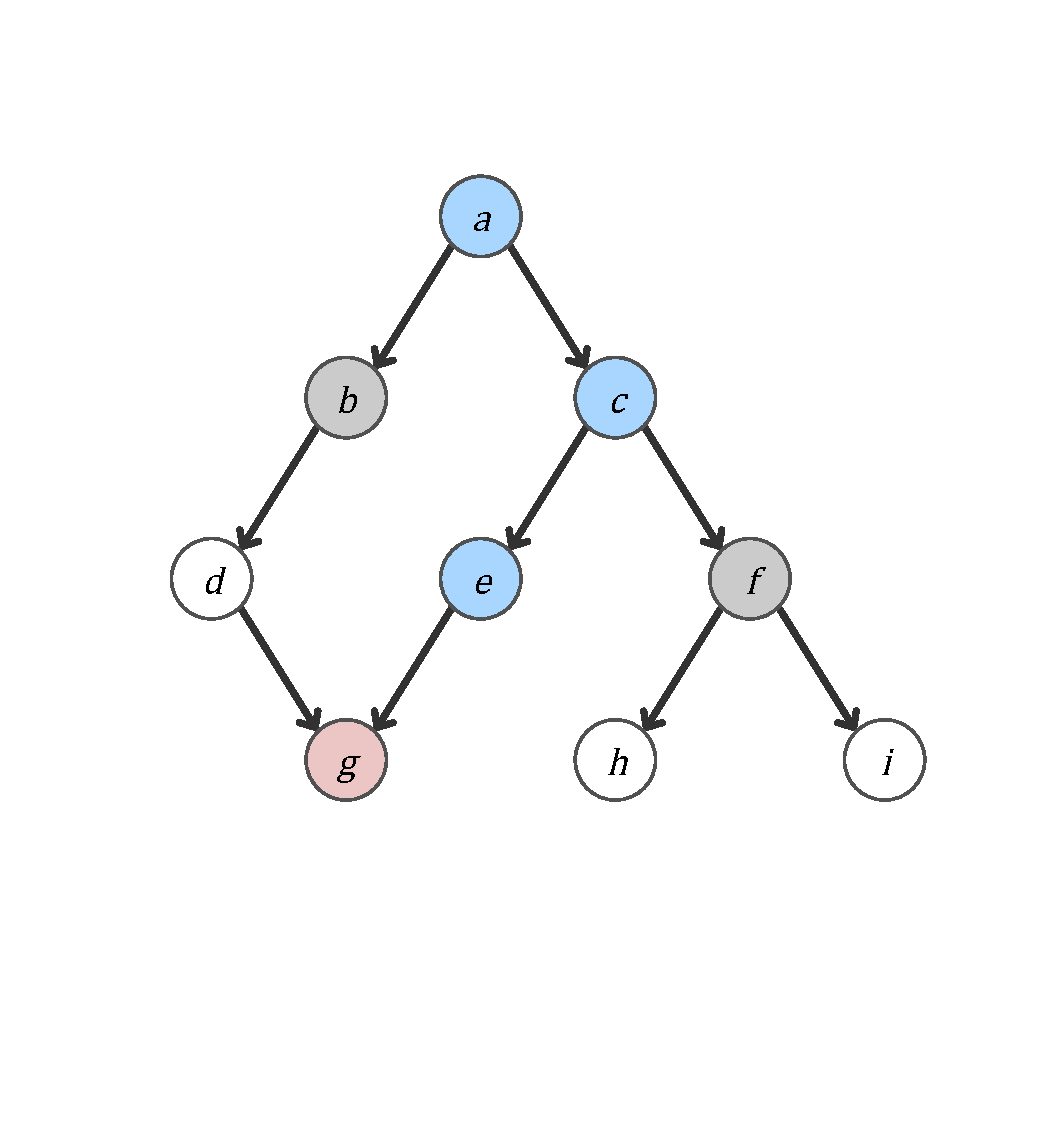
\includegraphics[scale=0.6]{Figures/rumi/full_joint_ontology}


\caption[A graph of terms illustrating different vertices used to calculate a full joint probability ]{ A directed acyclic graph representing the relationships between terms in an ontology. True term, or $T$, are represented by blue colored vertices: $\{ a, c, e\}$. The children of true terms, $\mathcal{C}(T)$, are denoted by grey and light-red vertices: $\{ b, f, g\}$. Terms which do not contribute anything to the full joint probability are shown in white and light-red: $\{d, g, h, i\}$. Term $g$ is colored light red to point out a special case when calculating the full joint probability of a graph.  Although one of term $g$'s parents are true, because it has one false parent it will not contribute to the calculation of the full joint probability because the probability it is false is always equal to one (\Cref{tab:rumiCPD}). All blue and grey terms taken together comprise the \emph{markov blanket} of $T$ and are necessary when calculating the full joint probability of a configuration, or combination of true and false values for all terms, in $\mathbf{V}$.}
\end{centering}
\label{fig:fulljoint}
\end{figure}

%%%%%%%%%%%%%%%%%%%%%%
%%%%%%%%%%%%%%%%%%%%%%

%Table
%%%%%%%%%%%%%%%%%%%%%%
%%%%%%%%%%%%%%%%%%%%%%

\begin{table*}[t]
\caption[A table of the joint probability distribution for variable $g$]{A table showing a conditional probability distribution for term $g$ from \Cref{fig:fulljoint}.  The purpose of this table is to illustrate how the consistency requirement affects joint probability tables in the bayesian network.   If at least one of a term's parents are false it is guaranteed that term is also false.  This is shown by considering the last three rows in the table.  
}

{\begin{tabular}{cc|cc}
\hphantom & \multicolumn{1}{c}{\hphantom} & \multicolumn{2}{c}{$\Pr(g)$}\\
$d$ & $e$ & True & False\\
\hline
True & True & .7 & .3\\
True & False & 0 & 1\\
False & True & 0 & 1\\
False & False & 0 & 1\\

\end{tabular}}
\label{tab:rumiCPD}
\end{table*}
%%%%%%%%%%%%%%%%%%%%%%
%%%%%%%%%%%%%%%%%%%%%%

The scope of terms considered can be reduced when calculating the joint probability of a configuration of $\mathbf{V}$ without affecting the final probability value. Because of the enforced consistency requirement (i.e. all ancestors of true terms are true; all descendants of false terms are false) the full joint probability of a configuration of the ontology, $\mathbf{V}$, can be calculated by considering only terms whose parents are all true. \Cref{eq:full_joint1} can be rewritten as

\begin{equation}
\Pr(\mathbf{V})=\underset{v\in T \cup \mathcal{C}(T)}{\prod}\Pr(v|\mathcal{P}(v)),
\label{eq:full_joint}
\end{equation}

\noindent where $T$ denotes all terms in $\mathbf{V}$ that are true, $\mathcal{C}(T)$ defines the children of all terms in $T$ (specifically, false terms all of whose parents are true), and  $T \cup \mathcal{C}(T)$ defines the unique union of the two sets. 

The derivation of \Cref{eq:full_joint} can be obtained by considering \Cref{fig:fulljoint} which illustrates a sample ontology with $9$ terms and \Cref{tab:rumiCPD} which represents the conditional probability distribution, or table, for vertex $g$.  If we write the joint probability of $\mathbf{V}$ using \Cref{eq:full_joint1} we obtain 
\begin{eqnarray*}
\Pr(\mathbf{V}) &= &\Pr(a=1) \times \Pr(b=0|a=1) \times \Pr(c=1|a=1) \times \Pr(d=0|b=0)\\
 & &  \times \Pr(e=1|c=1) \times \Pr(f=0|c=1) \times \Pr(g=0|d=0,e=1)\\
  & & \times \Pr(h=0|f=0) \times \Pr(i=0|f=0).
\end{eqnarray*}
First, we see that terms $h$ and $i$ contribute nothing to the joint probability because the probability a term is false given its parents are all false is always equal to 1.  Although $b$, and $f$ are false, because one of their parents are true the resulting probability is not 1.  Term $g$ can also be ignored because one of its parents is false.  For example, consider \Cref{tab:rumiCPD}, which shows the conditional probability table of term $g$.  If we consider instances where one of $g$'s parents are false we see that the resulting values are guaranteed to be 1. The resulting joint probability can subsequently be rewritten as 
\begin{eqnarray*}
\Pr (\mathbf{V}) & = &\Pr(a=1) \times \Pr(b=0|a=1) \times \Pr(c=1|a=1)\\  
 & & \times \Pr(e=1|c=1) \times \Pr(f=0|c=1).
\end{eqnarray*}

Because in practice most annotations only draw upon a small fraction of terms, most terms and their descendants, will be negative and will not contribute to the calculation of a given joint probability.  For this reason, although calculating the full joint probability has an asymptotic upper bound defined by the number of terms in the ontology, in practice it should have much lower complexity.

In this context, we are only interested in marginal probabilities that a protein is experimentally associated with a consistent subgraph $T$ in the ontology. This probability can be expressed as

\begin{equation}
\Pr(T)=\underset{v\in T}{\prod}\Pr(v|\mathcal{P}(v)).
\label{eq:factorization}
\end{equation}

\Cref{eq:factorization} can be derived from the full joint factorization by first marginalizing over the leaves of the ontology and then moving towards the root(s) for all nodes not in $T$.  

Although marginalizing over all negative terms gives a formulation that deviates from calculating the full joint probability it both simplifies calculating the information content of a sub-graph and can be philosophically justified. Unobserved annotations are only putative negative observations because explicit negative annotations are rarely deposited in biological databases.  In ignoring all negative terms we are implicitly recognizing that they are simply unobserved variables and not actual negative annotations.  

%%%%%%%%%%%%%%%%%%%%%%
%%%%%%%%%%%%%%%%%%%%%%
\subsection{Calculating the information content of a graph}
%%%%%%%%%%%%%%%%%%%%%%
%%%%%%%%%%%%%%%%%%%%%%

Now that we have properly defined the joint probability of a set of terms, or subgraph of the ontology, calculating the information content of those terms is relatively straightforward.  The information content of a subgraph can be thought of as the number of bits of information one would receive about a protein if it were annotated with that particular subgraph. We calculate the information content of a subgraph $T$ in a straightforward manner as

\[
i(T)=\log\frac{1}{\Pr(T)}
\]


\noindent and use a base 2 logarithm as a matter of convention. The information content of a subgraph $T$ can now be expressed by combining the previous two equations as

\begin{eqnarray*}
i(T) & = & \underset{v\in T}{\sum}\log\frac{1}{\Pr(v|\mathcal{P}(v))}\\
 & = & \underset{v\in T}{\sum}ia(v),
\end{eqnarray*}


\noindent where, to simplify the notation, we use $ia(v)$ to represent the negative logarithm of $\Pr(v|\mathcal{P}(v))$. Term $ia(v)$ can be thought of as the increase, or accretion, of information obtained by adding a child term to a parent term, or set of parent terms, in an annotation. We will refer to $ia(v)$ as \emph{information accretion} (perhaps information gain would be a better term, but because it is frequently used in other applications to describe an expected reduction in entropy, we avoid it in this situation).

A simple ontology containing five terms together with a conditional probability table associated with each node is shown in \Cref{fig:ontologytable}A. Note that because of the graph consistency requirement, each conditional probability table is limited to a single number. For example, at node $b$ in the graph, the probability $\Pr(b=1|a=1)$ is the only one necessary because $\Pr(b=0|a=1)=1-\Pr(b=1|a=1)$ and because $\Pr(b=1|a=0)$ is guaranteed to be $0$. In \Cref{fig:ontologytable}B we show a sample data set of four proteins functionally annotated according to the distribution defined by the Bayesian network. In \Cref{fig:ontologytable}C, we show the total information content for each of the four annotation graphs.

\begin{figure}
\noindent \begin{centering}
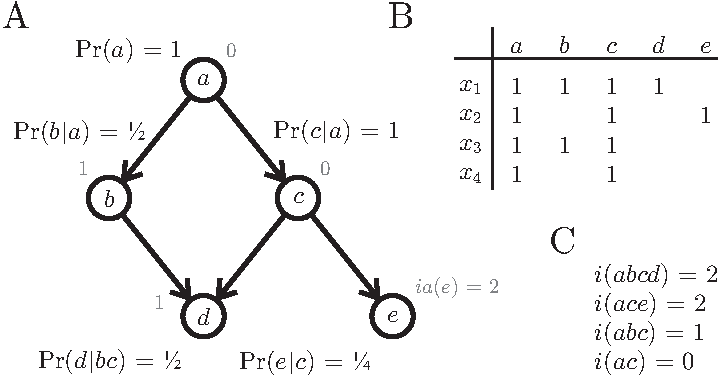
\includegraphics[scale=0.7]{Figures/rumi/ontology_table_v04}
\par\end{centering}

\caption[A sample ontology and data set illustrating calculating information content]{An example of an ontology, data set, and calculation of information content. (A) An ontology viewed as a Bayesian network together with a conditional probability table assigned to each node. Each conditional probability table is limited to a single number due to the consistency requirement in assignments of protein function. Information accretion calculated for each node, e.g. $ia(e)=-\log\Pr(e|c)=2$, are shown in grey next to each node. (B) A data set containing four proteins whose functional annotations are generated according to the probability distribution from the Bayesian network. (C) The total information content associated with each protein found in panel B; e.g. $i(ace)=ia(a)+ia(c)+ia(e)=2$. Note that $i(ab)=1$ and $i(abcde)=4$ although proteins with such annotation have not been observed in part B.}
\label{fig:ontologytable}
\end{figure}




%%%%%%%%%%%%%%%%%%%%%%
%%%%%%%%%%%%%%%%%%%%%%
\subsection{Comparing two annotation graphs}
%%%%%%%%%%%%%%%%%%%%%%
%%%%%%%%%%%%%%%%%%%%%%


We now consider a situation in which a protein's true and predicted function are represented by graphs $T$ and $P$, respectively. We define two metrics that can be thought of as the information-theoretic analogs of recall and precision, and refer to them as remaining uncertainty and misinformation, respectively. 

\textbf{Definition 1.} The \emph{remaining uncertainty} about the protein's true annotation corresponds to the information about the protein that is not yet provided by the graph $P$. More formally, we express the remaining uncertainty ($ru$) as

\begin{equation}
ru(T,P)=\underset{v\in T\setminus P}{\sum}ia(v),
\label{eq:ruSIMP}
\end{equation}


\noindent which is simply the total information content of the nodes in the ontology that are contained in true annotation $T$ but not in the predicted annotation $P$. Note that, in a slight abuse of notation, we apply set operations to graphs to manipulate only the vertices of these graphs. %which also indicates that the consistent graphs are treated here as sets of (weighted) nodes or functional terms. 

\textbf{Definition 2.} The \emph{misinformation} introduced by the classifier corresponds to the total information content of the nodes along incorrect paths in the prediction graph $P$. More formally, the misinformation is expressed as

\begin{equation}
mi(T,P)=\underset{v\in P\setminus T}{\sum}ia(v),
\label{eq:miSIMP}
\end{equation}


\noindent which quantifies how misleading a predicted annotation is. 

Here, a perfect prediction (one that achieves $P=T$) leads to $ru(T,P)=mi(T,P)=0$.  However, both $ru(T,P)$ and $mi(T,P)$ can be infinite in the limit. In practice, though, $ru(T,P)$ is bounded by the information content of the particular annotation, while $mi(T,P)$ is only limited by the number of annotations a predictor chooses to return. 


To illustrate calculation of remaining uncertainty and misinformation, in Figure 2 we show a sample ontology where the true annotation of a protein $T$ is determined by the two leaf terms $t_{1}$ and $t_{2}$, whereas the predicted subgraph $P$ is determined by the leaf terms $p_{1}$ and $p_{2}.$ The remaining uncertainty $ru(T,P)$ and misinformation $mi(T,P)$ can now be calculated by adding the information accretion corresponding to the nodes circled in grey. 

Finally, this framework can be used to define the similarity between the protein's true annotation and the predicted annotation without relying on identifying an individual common ancestor between pairs of leaves (this node is usually referred to as the maximum informative common ancestor; \citealt{Guzzi2012}). The information content of the subgraph shared by $T$ and $P$ is one such possibility; i.e. 
\[
s(T,P)=\underset{v\in T\cap P}{\sum}ia(v).
\]
%\textcolor{blue}{We define the similarity between the two sets as the information content of the common subgraph shared by them. More formally, we define this similarity as $s(T,P)=\underset{v\in T\cap P}{\sum}ia(v)$.}


%%%%%%%%%%%%%%%%%%%%%%
%%%%%%%%%%%%%%%%%%%%%%
\begin{figure}
\begin{centering}
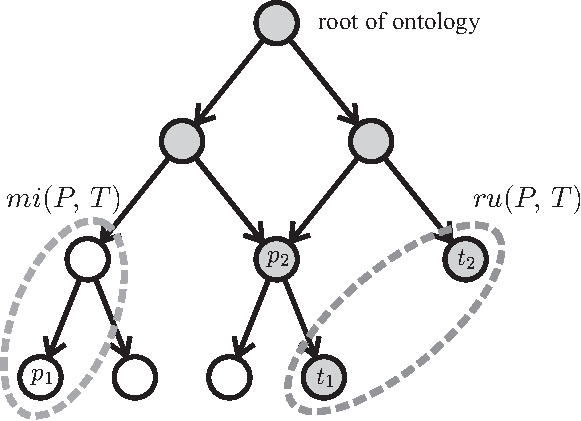
\includegraphics[scale=0.7]{Figures/rumi/ontology-rumi_v04}
\par\end{centering}

\caption[A graph showing terms used to calculate $ru$ and $mi$]{Illustration of calculating remaining uncertainty and misinformation given a predicted annotation graph $P$ and a graph of true annotations $T$. Graphs $P$ and $T$ are uniquely determined by the leaf nodes $p_{1}$, $p_{2}$, $t_{1}$, and $t_{2}$, respectively. Nodes colored in grey represent graph $T$. Nodes circled in grey are used to determine remaining uncertainty ($ru$; right side) and misinformation ($mi$; left side) between $T$ and $P$}.

\end{figure}
%%%%%%%%%%%%%%%%%%%%%%
%%%%%%%%%%%%%%%%%%%%%%


%%%%%%%%%%%%%%%%%%%%%%
%%%%%%%%%%%%%%%%%%%%%%
\subsection{Measuring the quality of function prediction}
%%%%%%%%%%%%%%%%%%%%%%
%%%%%%%%%%%%%%%%%%%%%%

A typical predictor of protein function usually outputs scores that indicate the strength (e.g. posterior probabilities) of predictions for each term in the ontology. To address this situation, the concepts of remaining uncertainty and misinformation need to be considered as a function of a decision threshold $\tau$. In such a scenario, predictions with scores greater than or equal to $\tau$ are considered positive predictions, while the remaining associations are considered negative (if the strength of a prediction is expressed via P-values or e-values, values lower than the threshold would indicate positive predictions). Regardless of the situation, every decision threshold results in a separate pair of values corresponding to the remaining uncertainty $ru(T,P(\tau))$ and misinformation $mi(T,P(\tau))$. 

The remaining uncertainty and misinformation for a previously unseen protein can be calculated as expectations over the data generating probability distribution. Practically, this can be performed by averaging over the entire set of proteins used in evaluation, i.e.

\begin{equation}
ru(\tau)=\frac{1}{n}\sum_{i=1}^{n}ru(T_{i},P_{i}(\tau))\label{eq:average_ru}
\end{equation}


\noindent and

\begin{equation}
mi(\tau)=\frac{1}{n}\sum_{i=1}^{n}mi(T_{i},P_{i}(\tau))\label{eq:average_mi}
\end{equation}


\noindent where $n$ is the number of proteins in the data set, $T_{i}$ is the true set of terms for protein $x_{i}$, and $P_{i}(\tau)$ is the set of predicted terms for protein $x_{i}$ given decision threshold $\tau$. Note that once the set of terms with scores greater than or equal to $\tau$ is determined, the set $P_{i}(\tau)$ is composed of the unique union of the ancestors of all predicted terms. As the decision threshold is moved from its minimum to its maximum value, the pairs of $(ru(\tau),mi(\tau))$ will result in a curve in 2D space. We refer to such a curve using $(ru(\tau),mi(\tau))_{\tau}$. Removing the normalizing constant ($\frac{1}{n}$) from the above equations would result in the total remaining uncertainty and misinformation associated with a database of proteins and a set of predictions.


%%%%%%%%%%%%%%%%%%%%%%
%%%%%%%%%%%%%%%%%%%%%%
\subsection{Weighted metrics}
%%%%%%%%%%%%%%%%%%%%%%
%%%%%%%%%%%%%%%%%%%%%%

One disadvantage of definitions in Equations \ref{eq:average_ru} and \ref{eq:average_mi} is that an equal weight is given to proteins with low and high information content annotations when averaging. To address this we assign a weight to each protein according to the information content of its experimental annotation. This formulation naturally downweights proteins with less informative annotations compared to proteins with rare, and therefore more informative (surprising), annotations. In biological data sets, frequently seen annotations have a tendency to be incomplete or shallow annotation graphs and arise due to the limitations or high-throughput nature of some experimental protocols. We define \emph{weighted remaining uncertainty} as

\begin{equation}
wru(\tau)=\frac{\sum_{i=1}^{n}i(T_{i})\cdot ru(T_{i},P_{i}(\tau))}{\sum_{i=1}^{n}i(T_{i})}
\label{eq:weighted_ru}
\end{equation}

\noindent and \emph{weighted misinformation} as

\begin{equation}
wmi(\tau)=\frac{\sum_{i=1}^{n}i(T_{i})\cdot mi(T_{i},P_{i}(\tau))}{\sum_{i=1}^{n}i(T_{i})}
\label{eq:weighted_mi}
\end{equation}


%\noindent \sout{A curve in the 2D space $(wru(\tau),wmi(\tau))_{\tau}$ can now be plotted and used to quantify or visualize the prediction quality for different classification models.}

%%%%%%%%%%%%%%%%%%%%%%
%%%%%%%%%%%%%%%%%%%%%%
\subsection{Semantic distance}
%%%%%%%%%%%%%%%%%%%%%%
%%%%%%%%%%%%%%%%%%%%%%

Finally, to provide a single performance measure which can be used to rank and evaluate protein function prediction algorithms, we introduce \emph{semantic distance} as the minimum distance from the origin to the curve $(ru(\tau),mi(\tau))_{\tau}$. More formally, the semantic distance $S_{k}$ is defined as

\begin{equation}
S_{k}=\underset{\tau}{\min}(ru^{k}(\tau)+mi^{k}(\tau))^{\frac{1}{k}},
\label{eq:semantic_distance}
\end{equation}

\noindent where $k$ is a real number $\ge 1$. Setting $k=2$ results in the minimum Euclidean distance from the origin. The preference for Euclidean distance ($k=2$) over say Manhattan distance ($k=1$) is to penalize unbalanced predictions with respect to the depth of predicted and experimental annotations. 

%\textcolor{blue}{One interesting property of $S_{k}$ is its relationship with the semantic measure proposed by \cite{Jiang1997}.  If one replaces $i(T)$ and $S(T,P)$ with our graph based definitions of information content and similarity, then we state, without proof, that $S_{k}$ is equivalent to Jiang and Conrath's metric when $k=1$.}

%%%%%%%%%%%%%%%%%%%%%%
%%%%%%%%%%%%%%%%%%%%%%
\subsection{Precision and recall}
%%%%%%%%%%%%%%%%%%%%%%
%%%%%%%%%%%%%%%%%%%%%%

In order to contrast the semantic distance-based evaluation with more conventional performance measures, in this section we briefly introduce precision and recall for measuring functional similarity. As before, we consider a set of propagated experimental terms $T$ and predicted terms $P(\tau)$, and define precision as the fraction of terms predicted correctly. More specifically, 

\[
pr(T,P(\tau))=\frac{|T\cap P(\tau)|}{|P(\tau)|},
\]

\noindent where $\left|\cdot\right|$ is the set cardinality operator.  Only proteins for which the prediction set is non-empty can be used to calculate average precision.  To address this issue the root term is counted as a prediction for all proteins. Similarly, recall is defined as the fraction of experimental (true) terms which were correctly predicted, i.e.

\[
rc(T,P(\tau))=\frac{|T\cap P(\tau)|}{|T|}.
\]


\noindent As before, precision $pr(\tau)$ and recall $rc(\tau)$ for the entire data set are calculated as averages over the entire set of proteins (note that an alternative definition of precision and recall given by \citealt{Verspoor2006} is described in \Cref{sec:rumiAddTop}). Finally, to provide a single evaluation measure we use the maximum F-measure over all decision thresholds. For a particular set of terms $T$ and $P(\tau)$, F-measure is calculated as the harmonic mean of precision and recall. More formally, the final evaluation metric is calculated as

\begin{equation}
F_{\max}=\underset{\tau}{\max}\left\{ 2\cdot\frac{pr(\tau)\cdot rc(\tau)}{pr(\tau)+rc(\tau)}\right\} 
\label{eq:fmax}
\end{equation}


\noindent where $pr(\tau)$ and $rc(\tau)$ are calculated by averaging over the data set. 

%%%%%%%%%%%%%%%%%%%%%%
%%%%%%%%%%%%%%%%%%%%%%
\subsubsection{Information-theoretic weighted formulation}
%%%%%%%%%%%%%%%%%%%%%%
%%%%%%%%%%%%%%%%%%%%%%

The definition of information accretion and the use of a probabilistic framework defined by the Bayesian network enables the straightforward application of information accretion to weight each term in the ontology. Therefore, it is easy to generalize the definitions of precision and recall from the previous section into a weighted formulation. Here, weighted precision and weighted recall can be expressed as

\[
wpr(T,P(\tau))=\frac{\underset{v\in T\cap P(\tau)}{\sum}ia(v)}{\underset{v\in P(\tau)}{\sum}ia(v)}
\]


\noindent and

\[
wrc(T,P(\tau))=\frac{\underset{v\in T\cap P(\tau)}{\sum}ia(v)}{\underset{v\in T}{\sum}ia(v)}.
\]


\noindent  Weighted precision $wpr(\tau)$ and recall $wrc(\tau)$ can then be calculated as weighted averages over the database of proteins, as in Equations \ref{eq:weighted_ru} and \ref{eq:weighted_mi}.

In addition to weighted precision and recall our framework also facilitates calculating weighted specificity

\[
%wsp(T,P(\tau))=\frac{ \underset{v\in \stcomp{T} \cap \stcomp{P} }{\sum}ia(v)}{\underset{v\in \stcomp{T}}{\sum}ia(v)}
wsp(T,P(\tau))=\frac{\underset{v\in T^{\bf{c}} \cap P^{\bf{c}}(\tau)}{\sum}ia(v)}{\underset{v\in T^{\bf{c}}}{\sum}ia(v)}
\]
where $T^{\bf{c}}$ represents the complement of set $T$ ($G \setminus T$).

%%%%%%%%%%%%%%%%%%%%%%
%%%%%%%%%%%%%%%%%%%%%%
\subsection{Supplementary evaluation metrics}
\label{sec:rumisupmethods}
%%%%%%%%%%%%%%%%%%%%%%
%%%%%%%%%%%%%%%%%%%%%%

When calculating remaining uncertainty, misinformation, precision and recall only consistent subgraphs of the Gene Ontology were considered. Under this framework, if a protein is annotated with multiple terms (either experimentally determined or predicted), as in \Cref{fig:ontologytable} , we determine consistent graphs $T$ (true) or $P$ (predicted) by recursively propagating annotations towards the root(s) of the ontology and taking a union of all terms encountered along the way. In each of these measures, it is sufficient to only consider vertices (terms) in the annotation graphs and calculate the similarity measure by manipulating vertices in an additive fashion. For example, each vertex in $T$ or $P$ counts equally in the precision/recall-based evaluation while the information accretion is used to weight the vertices in the ru-mi-based evaluation. 

A distinctly different approach can be taken by considering, on an individual basis, each leaf term that comprises a set $T$ or $P$. This is the approach taken to calculate various information-theoretic metrics \citep{Resnik1995, Jiang1997, Lin1998, Lord2003, Schlicker2006} as well as to provide an alternative definition of precision and recall \citep{Verspoor2006}. In this context the sets of leaf terms that define $T$ and $P$ (which we refer to as $\mathcal{L}(T)$ and $\mathcal{L}(P)$ respectively, and formally introduce below) are used to calculate a given metric. After calculating all pairwise metrics between the leaf terms, several different methods for averaging these scores can be applied to create a single similarity (or distance) value between $T$ and $P$.  We discuss these approaches below.

%%%%%%%%%%%%%%%%%%%%%%
%%%%%%%%%%%%%%%%%%%%%%
\subsubsection{Basic definitions}
%%%%%%%%%%%%%%%%%%%%%%
%%%%%%%%%%%%%%%%%%%%%%

Suppose we are given an ontology in the form of directed acyclic graph $G=(V, E)$, where $V$ is a set of vertices and $E\subset V\times V$ is the set of edges. In this graph, given an edge $(u,v) \in E$, we refer to vertex $u$ as a parent of $v$ and, alternatively, to vertex $v$ as a child of $u$. We also consider a set of all ancestors of $v$, $\mathcal{A}(v)$, and find this set by recursively identifying parents of all discovered nodes starting with $v$ until the root(s) of the ontology is (are) reached. For mathematical convenience, we consider vertex $v$ to be a member of $\mathcal{A}(v)$. Finally, given two vertices $u$ and $v$, we define a set of common ancestor nodes between these two vertices as $\mathcal{A}(u,v)$. Thus, $\mathcal{A}(u,v)= \mathcal{A}(u)\cap \mathcal{A}(v)$.

Consider now a consistent annotation graph $T$, where the set of vertices in $T$ is a subset of vertices in $G$. We define $\mathcal{L}(T)$, or the set of leaf terms represented by $T$, as

\begin{equation}
\mathcal{L}(T)=\{u : u \in T \land \lnot\exists ( (u, v) \in E  \land v \in T)\}.
\end{equation}

\noindent
In other words, $\mathcal{L}(T)$ contains only those vertices (terms) from $T$ that do not have children in $T$. Thus, the leaf terms are defined with respect to a particular annotation graph $T$ and generally differ from the leaf nodes in the ontology. 

%%%%%%%%%%%%%%%%%%%%%%
%%%%%%%%%%%%%%%%%%%%%%
\subsubsection{Information-theoretic metrics between pairs of vertices}
%%%%%%%%%%%%%%%%%%%%%%
%%%%%%%%%%%%%%%%%%%%%%

When calculating the information\hyp{}theoretic metrics of \citet{Resnik1995}, \citet{Jiang1997}, \citet{Lin1998}, \citet{Lord2003}, and \citet{Schlicker2006}, we calculate the information content of an individual term $v \in V$ as

\begin{equation}
i(v)=\log\frac{1}{\Pr(v)}
\end{equation}

\noindent
where $\Pr(v)$ can be calculated as the relative frequency of term $v$ among experimentally annotated proteins. The similarity between two distinct terms $u$ and $v$ as defined by \citet{Resnik1995} was calculated as

\begin{equation}
s_{R}(u,v)=\underset{w\in \mathcal{A}(u,v)}{\max}\{i(w)\},
\end{equation}

\noindent where $\mathcal{A}(u, v)$, as mentioned above, defines the set of common ancestors of terms $u$ and $v$. Similarity as defined by \citet{Lin1998} was calculated as

\begin{equation}
s(u,v)=\frac{s_{R}(u,v)}{i(u)+i(v)},
\end{equation}

\noindent and as defined by \citet{Schlicker2006} as

\begin{equation}
s(u,v)=\frac{s_{R}(u,v)}{i(u)+i(v)}\cdot(1-\underset{w\in \mathcal{A}(u,v)}{\min}\{\Pr(w)\}).
\end{equation}

\noindent Finally, the distance metric defined by \citet{Jiang1997} was calculated as

\begin{equation}
d(u,v)=i(u)+i(v)-2 \cdot s_{R}(u,v).
\end{equation}

%%%%%%%%%%%%%%%%%%%%%%
%%%%%%%%%%%%%%%%%%%%%%
\subsubsection{Information-theoretic metrics between pairs of graphs}
\label{sec:averaging}
%%%%%%%%%%%%%%%%%%%%%%
%%%%%%%%%%%%%%%%%%%%%%


Since the above metrics are only defined for two distinct terms, it is necessary to provide a mechanism to utilize these metrics in instances where a protein is annotated with graphs containing multiple leaf terms. Given two non-empty consistent annotation graphs of true and predicted terms, $T$ and $P$, and the set of leaf terms that define each set, $\mathcal{L}(T)$ and $\mathcal{L}(P)$, we employed two strategies for averaging. In the first case values were averaged between all possible pairs of terms in $\mathcal{L}(T)$ and $\mathcal{L}(P)$. Specifically, we calculated $s(T,P)$ as 

\begin{equation}
s(T, P)=\frac{1}{|\mathcal{L}(T)|\cdot|\mathcal{L}(P)|}\underset{t\in\mathcal{L}(T)}{\sum}\underset{p\in\mathcal{L}(P)}{\sum}s(t,p).
\end{equation}

\noindent We refer to this form of averaging as \emph{all-pair} averaging. This method of averaging was applied by \citet{Lord2003} in calculating similarity between two functional annotations.

In the second case we calculated the similarity between the two sets as the average of the maximum similarity between a term from one set and all terms in the other.  Specifically, we calculated $s(T,P)$ as 

\begin{equation}
s(T, P)=\frac{1}{2|\mathcal{L}(T)|}\underset{t\in\mathcal{L}(T)}{\sum}\underset{p\in\mathcal{L}(P)}{\max}\{s(t,p)\}+\frac{1}{2|\mathcal{L}(P)|}\underset{p\in\mathcal{L}(P)}{\sum}\underset{t\in\mathcal{L}(T)}{\max}\{s(t, p)\}.
\label{eq:maxaverage}
\end{equation}

\noindent This measure represents the technique of averaging employed by \citet{Verspoor2006} when calculating precision and recall (originally referred to as hierarchical precision and recall). There, the authors separately calculate precision as

\begin{equation}
pr(T, P)=\frac{1}{|\mathcal{L}(P)|}\underset{p\in\mathcal{L}(P)}{\sum}\underset{t\in\mathcal{L}(T)}{\max}\frac{|\mathcal{A}(t,p)|}{|\mathcal{A}(p)|}
\end{equation}

\noindent and recall as

\begin{equation}
rc(T, P)=\frac{1}{|\mathcal{L}(T)|}\underset{t\in\mathcal{L}(T)}{\sum}\underset{p\in\mathcal{L}(P)}{\max}\frac{|\mathcal{A}(t,p)|}{|\mathcal{A}(t)|}.
\end{equation}

\noindent We refer to this method of averaging as \emph{max-average}. Although not implemented here, \citet{Schlicker2006} employ a technique for averaging that is similar to \Cref{eq:maxaverage}, but takes the maximum average similarity for one set as opposed to the average between the two. Specifically,

\begin{equation}
s(T, P)=\max \left\{ \frac{1}{|\mathcal{L}(T)|}\underset{t\in\mathcal{L}(T)}{\sum}\underset{p\in\mathcal{L}(P)}{\max}\{s(t,p)\},\frac{1}{|\mathcal{L}(P)|}\underset{p\in\mathcal{L}(P)}{\sum}\underset{t\in\mathcal{L}(T)}{\max}\{s(t,p)\} \right\} 
\end{equation}

\noindent When averaging pairwise comparisons for distance metrics, the above averages are calculated as the average of minimum pairwise distances instead of maximum pairwise similarities.  

%%%%%%%%%%%%%%%%%%%%%%
%%%%%%%%%%%%%%%%%%%%%%
\subsection{Additional topological metrics}
\label{sec:rumiAddTop}
%%%%%%%%%%%%%%%%%%%%%%
%%%%%%%%%%%%%%%%%%%%%%

In addition to information-theoretic metrics, we also used Jaccard's similarity coefficient \citep{jaccard1901} when calculating the similarity between the two consistent annotation graphs $T$ and $P$. The Jaccard similarity coefficient is defined as

\begin{equation}
s(T,P)=\frac{|T\cap P|}{|T\cup P|}.
\end{equation}

\noindent We note that cosine similarity as well as Maryland bridge coefficient \citep{Glazko2005} usually result in values correlated with the Jaccard similarity coefficient. For that reason, these two similarity measures were not presented.



%%%%%%%%%%%%%%%%%%%%%%
%%%%%%%%%%%%%%%%%%%%%%

%%%%%%%%%%%%%%%%%%%%%%
%%%%%%%%%%%%%%%%%%%%%%
\section{Confusion matrix interpretation of $ru$ and $mi$}
%%%%%%%%%%%%%%%%%%%%%%
%%%%%%%%%%%%%%%%%%%%%%
While we introduce remaining uncertainty and misinformation in the context of comparing sub graphs of a larger ontology these two terms can also be intuitively interpreted as the information theoretic analogs of false positives and false negatives or Type I and Type II errors.  If we consider the confusion matrix in \Cref{tab:rumiCONF} we see the four positive outcomes that can occur when attempting to perform binary classification.  False positives (Type I errors) are instances where a data point is a negative example but is incorrectly classified as a positive.  In the context of hypothesis testing these are cases where the null hypothesis is true, but has incorrectly been rejected.  False negatives (Type II errors) represent cases where the data point is a positive, but has incorrectly been labeled as a negative (false negatives).  These are cases where the null hypothesis is false, but a model has failed to reject it.  

Given a set of true terms, $T$, and predicted terms, $P$, then $P\setminus T$ would represent the terms that would fall in the false positive or Type I error portion of the confusion matrix.  As defined in \Cref{eq:miSIMP}, this is the same set of terms whose joint probability, and subsequently information content, are measured when calculating misinformation.  In this context, misinformation can be thought of as the number of bits of information, instead of traditional counts, the false positives represent. Conversely, the if we consider false negatives, or the set of terms defined by $T\setminus P$ we are referring to the same set of terms used to calculate remaining uncertainty in \Cref{eq:ruSIMP}.  

%Table
%%%%%%%%%%%%%%%%%%%%%%
%%%%%%%%%%%%%%%%%%%%%%

\begin{table*}[t]
\caption[A confusion matrix]{A sample confusion matrix showing the four potential outcomes when performing binary classification.
\label{tab:rumiCONF}}
{
\begin{tabular}{l|l|c|c|}
\multicolumn{2}{c}{}&\multicolumn{2}{c}{True label}\\
\cline{3-4}
\multicolumn{2}{c|}{}&Positive & Negative\\
\cline{2-4}
\multirow{2}{*}{Predicted label} & Positive & True positives & False positives\\
\cline{2-4} 
& Negative & False negatives & True negatives\\
\cline{2-4}
\end{tabular}}{}

\end{table*}
%%%%%%%%%%%%%%%%%%%%%%
%%%%%%%%%%%%%%%%%%%%%%

%%%%%%%%%%%%%%%%%%%%%%
%%%%%%%%%%%%%%%%%%%%%%





\section{Analysis of semantic distance}
It is desirable to show that $S_{k}(T_{1},T_{2})$ is a metric. This is well known for $k=1$ \citep{deza2013}, but we wish to extend the proof to larger values of $k$.

In order to rove that $S_{k}(T_{1},T_{2})$ is a metric we first represent the terms associated with a set of sequences using a venn diagram (\Cref{fig:sdvenn}) where $p$, $q$, $s$, and $t$ each represent a mutually exclusive and collective exhaustive subsets of terms in $T_{1}$, (where any of these sets may be the empty set) , and similarly define $T_{2}=\{q, r, t, u\}$, we can rewrite \Cref{eq:semantic_distance} as

\[
S_{k}(T_{1},T_{2})=\left( \left[ \underset{t\in p \cup s}{\sum} ia(t) \right]^{k} + \left[ \underset{t\in r \cup u}{\sum} ia(t) \right]^{k} \right)^{1/k}
\]

In an abuse of notation where we simply refer to the sum of $ia$ values for terms in each set as the set itself, the above equation can be further simplified and written as

\[
S_{k}(T_{1},T_{2})=\left( \left[ p+s\right]^{k} + \left[ r+u\right]^{k} \right)^{1/k}
\]


%%%%%%%%%%%%%%%%%%%%%%
%%%%%%%%%%%%%%%%%%%%%%
\begin{figure*}[h!]
\begin{centering}
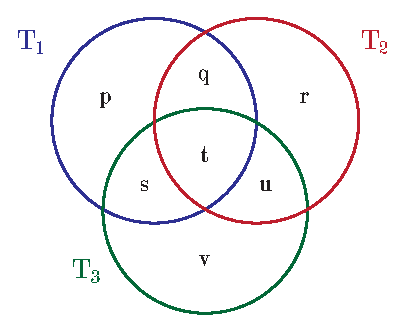
\includegraphics[width=0.45\linewidth]{Figures/sdproof/venn}
\par\end{centering}
\caption[A Venn diagram]{A Venn diagram showing the subsets of terms used to calculate the semantic distance between three pairs of annotations, $T_{1}$, $T_{2}$, and $T_{3}$. }
\label{fig:sdvenn}
\end{figure*}
%%%%%%%%%%%%%%%%%%%%%%
%%%%%%%%%%%%%%%%%%%%%%



\begin{theorem}
$S_{k}$ between two sets of terms, $T_{1}$ and $T_{2}$, is a metric for any real number $k \geq 1$.
\end{theorem}

\begin{proof}
%\begin{lemma}[Non-negativity]

~\begin{itemize}

\item \emph{Non-negativity}\\
The non-negativity of $S_{k}(T_{1},T_{2})$ is ensured by the fact that the information accretion, $ia(t)$, of an individual term is non-negative.  Because the conditional probability of a term given its parents, $\Pr (t|parents)$ is always $\geq 0$ and $\leq 1$, by virtue its information accretion, $-\log (t|parents)$, is always non-negative.
%\end{lemma}

%\begin{lemma}[Identity and indiscernibility]

\item \emph{Identity and indiscernibility}\\
$T_{1}=T_{2}$ if and only if $S_{k}(T_{1},T_{2})=0$.  First, if $T_{1}=T_{2}$, then $p, s, r, u = \varnothing$, and the resulting $ru(T_{1},T_{2})$, $mi(T_{1},T_{2})$, and $S_{k}(T_{1},T_{2})$ values will be zero.  Second, if $S_{k}(T_{1},T_{2})=0$ we know that $T_{1}=T_{2}$.  This is because the sum of information accretion values for any combination of terms will always be greater than zero, the only way that $ru(T_{1},T_{2})$ and $mi(T_{1},T_{2})$ can be equal to zero is when $p, s, r, u = \varnothing$.  When these sets are empty, it must be the case that $T_{1}=T_{2}$; and all terms in $T_{1}$ and $T_{2}$ are the same.
%\end{lemma}

%\begin{lemma}[Symmetry]
\item \emph{Symmetry}\\
$S_{k}(T_{1},T_{2})=S_{k}(T_{2},T_{1})$ because of the commutative property of addition, and the symmetric nature of $ru$ and $mi$.  For example, it can be shown that 
\[
ru(T_{1},T_{2}) = mi(T_{2},T_{1}),
\]
because $(p+s)=(p+s)$.
%\end{lemma}

%\begin{lemma}[Triangle inequality]
\item \emph{Triangle inequality}\\
Here we prove that $S_{k}(T_{1}, T_{2})+S_{k}(T_{1},T_{3}) \geq S_{k}(T_{2},T_{3})$ by showing that
\[
\left[\left(p+s\right)^{k}+\left(r+u\right)^{k}\right]^{\frac{1}{k}}+\left[\left(p+q\right)^{k}+\left(v+u\right)^{k}\right]^{\frac{1}{k}}\geq\left[\left(q+r\right)^{k}+\left(s+v\right)^{k}\right]^{\frac{1}{k}}
\]
where all elements are non-negative.
In order to prove this we rely on the Minkowski inequality, which can be expressed as

\[
 \left(\sum\limits_{i=1}^{n}  a_{i}^k \right)^{1/k} + \left(\sum\limits_{i=1}^{n}  b_{i}^k \right)^{1/k} \geq \left( \sum\limits_{i=1}^{n} \left[ a_{i} + b_{i} \right]^{k} \right)^{1/k}, 
\]

%The Minkowski inequality (which holds for $k\geq1$) is applied to theleft-hand side to obtain
where, for the sake of simplicity absolute value symbols have been omitted.  We first modify the left-hand side, using the Mikowski inequality,
\[
\left[\left(p+s\right)^{k}+\left(r+u\right)^{k}\right]^{\frac{1}{k}}+\left[\left(p+q\right)^{k}+\left(v+u\right)^{k}\right]^{\frac{1}{k}}\geq\left[\left(r+u+p+q\right)^{k} +  \left(p+s+v+u\right)^{k} \right]^{\frac{1}{k}},
\]
by setting the set $a = ( r+u , p+s )$ and $b = ( p+q, v+u )$.

Since we know that inequalities are transitive (i.e. if $a>b$ and $b>c$ then $a>c$), and it can be shown that

\[
\left[\left(r+u+p+q\right)^{k} +  \left(p+s+v+u\right)^{k} \right]^{\frac{1}{k}}\geq\left[\left(q+r\right)^{k}+\left(s+v\right)^{k}\right]^{\frac{1}{k}},
\]
the original formula has been proven.


%\end{lemma}
\end{itemize}
\end{proof}


%%%%%%%%%%%%%%%%%%%%%%
%%%%%%%%%%%%%%%%%%%%%%


%%%%%%%%%%%%%%%%%%%%%%
%%%%%%%%%%%%%%%%%%%%%%
\section{Annotation models}
%%%%%%%%%%%%%%%%%%%%%%
%%%%%%%%%%%%%%%%%%%%%%

We first collected all proteins with GO annotations supported by experimental evidence codes (EXP, IDA, IPI, IMP, IGI, IEP, TAS, IC) from the January 2011 version of the Swiss-Prot database (29,699 proteins in MFO; 31,608 in BPO; and 30,486 in CCO). We then generated three simple function annotation models: Na\"ive, BLAST and GOtcha, in order to assess the ability of performance metrics to accurately reflect the quality of a predicted set of annotations. In addition to these three methods, we generated another set of ``predictions" by collecting experimental annotations for the same set of proteins from a database generated by the GO Consortium released at about the same time as our version of Swiss-Prot. This was done to quantify the variability of experimental annotation across different databases using the same set of metrics. In addition, this comparison can be used to estimate the empirical upper limit of prediction accuracy because the observed performance is limited by the noise in experimental data. All computational methods were evaluated using 10-fold cross-validation. 

%%%%%%%%%%%%%%%%%%%%%%
%%%%%%%%%%%%%%%%%%%%%%
\subsection{The Na\"ive model}
\label{sec:naive}
%%%%%%%%%%%%%%%%%%%%%%
%%%%%%%%%%%%%%%%%%%%%%

The Na\"ive model was designed to reflect biases in the distribution of terms in the data set and was the simplest annotation model we employed. It was generated by first calculating the relative frequency of each term in the training data set. This value was then used as the prediction score for every protein in the test set; thus, every protein in the test partition was assigned an identical set of predictions over all functional terms. The performance of the Na\"ive model reflects what one could expect when annotating a protein with no knowledge about that protein.

%%%%%%%%%%%%%%%%%%%%%%
%%%%%%%%%%%%%%%%%%%%%%
\subsection{The BLAST model}
\label{sec:blast}
%%%%%%%%%%%%%%%%%%%%%%
%%%%%%%%%%%%%%%%%%%%%%

The BLAST model was generated using local sequence identity scores to annotate proteins. Given a target protein sequence $x$, a particular functional term $v$ in the ontology, and a set of sequences $S_{v}=\{s_{1},s_{2},\ldots\}$ annotated with term $v$, we determine the BLAST predictor score for function $v$ as 

%$\max\left\{ sid(x,s):s\in S_{v}\right\} $, 

\[
\underset{s\in S_{v}}{\max}\left\{ sid(x,s)\right\}, 
\]

\noindent where $sid(x,s)$ is the maximum sequence identity returned by the BLAST package \citep{Altschul1997} when the two sequences are aligned. We chose this method to mimic the performance one would expect if they simply used BLAST to transfer annotations between similar sequences.

%%%%%%%%%%%%%%%%%%%%%%
%%%%%%%%%%%%%%%%%%%%%%
\subsection{The GOtcha model}
%%%%%%%%%%%%%%%%%%%%%%
%%%%%%%%%%%%%%%%%%%%%%

The third method, GOtcha \citep{Martin2004}, was selected to incorporate not only sequence identity between protein sequences, but also the structure of the ontology (technically, BLAST also incorporates structure of the ontology but in a relatively trivial manner). %The GOtcha method outputs so-called i-scores for every protein by cumulatively propagating scores toward the root of the ontology and then normalizing them. As such it is an inexpensive and robust predictor of function. %
Specifically, given a target protein $x$, a particular functional term $v$, and a set of sequences $S_{v}=\{s_{1},s_{2},\ldots\}$ annotated with function $v$, one first determines the r-score for function $v$ as 

\[
r_{v}=c - \sum_{s\in S_{v}}\log(e(x,s)), 
\]

\noindent where $e(x,s)$ represents the E-value of the alignment between the target sequence $x$ and sequence $s$, and $c=2$ is a constant added to the given quantity to ensure all scores were above 0. Given the r-score for function $v$, i-scores were then calculated by dividing the r-score of each function by the score for the root term $i_{v}=r_{v}/r_{root}$. As such, GOtcha is an inexpensive and robust predictor of function.




%%%%%%%%%%%%%%%%%%%%%%
%%%%%%%%%%%%%%%%%%%%%%


%%%%%%%%%%%%%%%%%%%%%%
%%%%%%%%%%%%%%%%%%%%%%
\section{Experiments and results}
%%%%%%%%%%%%%%%%%%%%%%
%%%%%%%%%%%%%%%%%%%%%%


In this section we fist analyze the average information content in a data set of experimentally annotated proteins and then evaluate performance accuracy of different function prediction methods using both topological and probabilistic metrics. Each experiment was conducted on all three categories of the Gene Ontology: Molecular Function (MFO), Biological Process (BPO), and Cellular Component (CCO) ontologies. In order to avoid cases where the information content of a term is infinite a pseudo-count of $1$ was added to each term, and the total number of proteins in the data set was incremented when calculating term frequencies.

%%%%%%%%%%%%%%%%%%%%%%
%%%%%%%%%%%%%%%%%%%%%%
\subsection{Average information content of a protein}
%%%%%%%%%%%%%%%%%%%%%%
%%%%%%%%%%%%%%%%%%%%%%

We first examined the distribution of the information content per protein for each of the three ontologies (Figure \ref{fig:rumi3}). We observe a wide range of information contents in all ontologies, reaching over 128 bits in case of BPO (which corresponds to a factor of 128 in the probability of observing particular annotation graphs). The distributions for MFO and CCO show unusual peaks for very low information contents, suggesting that a large fraction of annotation graphs in these ontologies are low quality. One such anomaly is created by the term 'binding' in MFO that is associated with 72\% of proteins. Furthermore, 41\% of proteins are annotated with its child `protein binding' as a leaf term, and 26\% are annotated with it as their sole leaf term. Such annotations, which are clearly a consequence of high-throughput experiments, present a significant difficulty in method evaluation.

%%%%%%%%%%%%%%%%%%%%%%
%%%%%%%%%%%%%%%%%%%%%%
\begin{figure*}[h!]
\begin{centering}
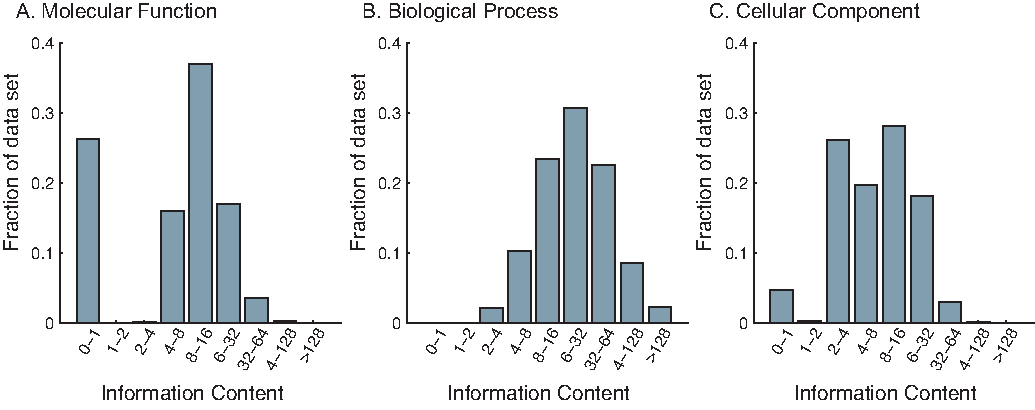
\includegraphics[width=0.85\linewidth]{Figures/rumi/Figure3}
\par\end{centering}
\caption[Distribution of information content (in bits) of protein experimental annotations]{Distribution of information content (in bits) over proteins annotated by terms for each of the three ontologies. The average information content of a protein was estimated at 10.9 (std. 10.2), 32.0 (std. 33.6), and 10.4 (std. 9.2) bits for MFO, BPO, and CCO, respectively.}
\label{fig:rumi3}
\end{figure*}
%%%%%%%%%%%%%%%%%%%%%%
%%%%%%%%%%%%%%%%%%%%%%


Previously, we showed that the distribution of leaf terms in protein annotation graphs exhibits scale-free tendencies \citep{Clark2011}. Here, we also analyzed the average number of leaf terms per protein and compared it with the information content of that protein. We estimate the average number of leaf terms to be 1.6 (std. 1.0), 3.0 (std. 3.6), and 1.6 (std. 1.0) for MFO, BPO, and CCO, respectively, and calculate Pearson correlation between the information content and the number of leaf terms for a protein (0.80, 0.92, and 0.71). Such high level of correlation suggests that proteins annotated with a small number of leaf terms are generally annotated by shallow graphs. This is particularly evident in the case of `protein binding' annotations that can be derived from yeast-2-hybrid experiments, but provide little insight into the functional aspects of these complexes when only viewed as GO annotations. We believe the wide range of information contents coupled with the fact that a large fraction of proteins were essentially uninformative, justifies the weighting proposed in this work.

%%%%%%%%%%%%%%%%%%%%%%
%%%%%%%%%%%%%%%%%%%%%%
\subsection{Two-dimensional plots}
%%%%%%%%%%%%%%%%%%%%%%
%%%%%%%%%%%%%%%%%%%%%%

In order to assess how each metric evaluated the performance of the four prediction methods we generated two-dimensional plots. Figure \ref{fig:rumi4} shows the performance of each predictor using precision/recall and ru-mi curves, as well as their weighted variants. The performance of the GO/Swiss-Prot annotation is represented as a single point because it compares two databases of experimental annotations where predictions are all binary and do not have associated scores.

%%%%%%%%%%%%%%%%%%%%%%
%%%%%%%%%%%%%%%%%%%%%%
\begin{figure*}[h!]
\begin{centering}
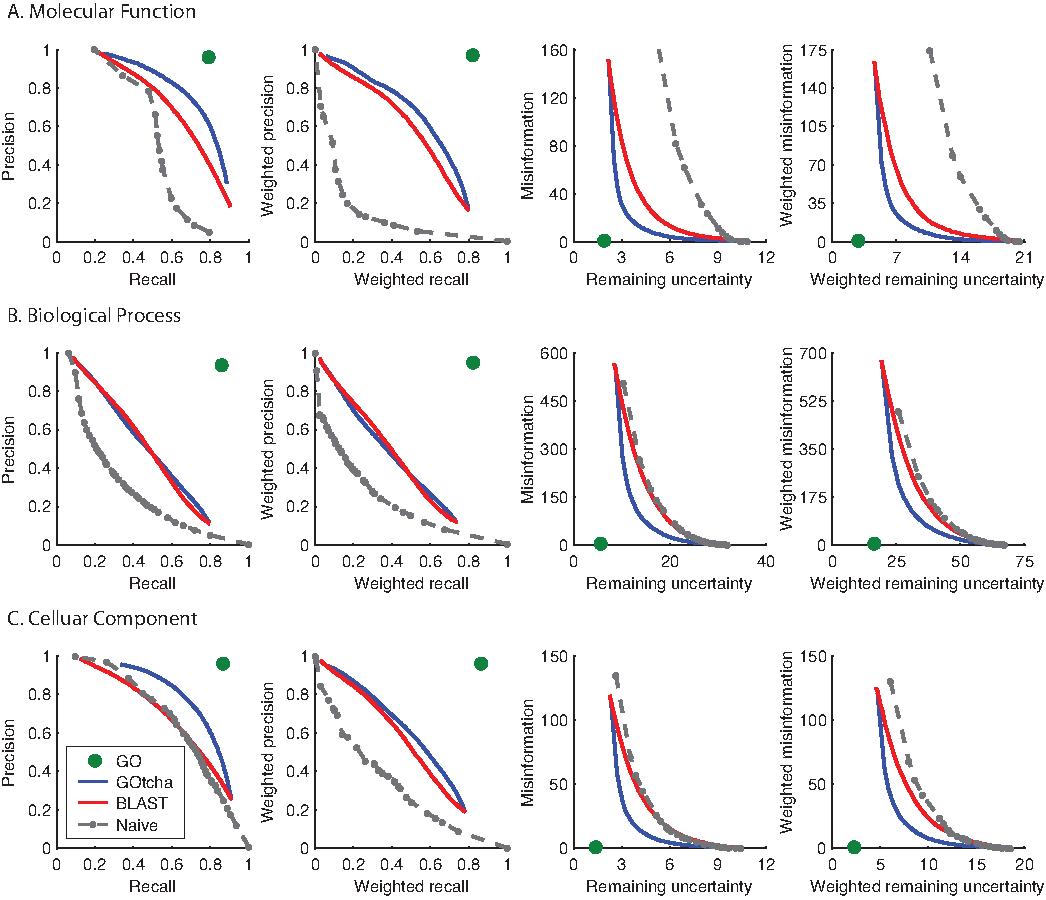
\includegraphics[width=\linewidth]{Figures/rumi/Figure4}
\end{centering}
\caption[Plots of $(pr(\tau),rc(\tau))_{\tau}$, $(wpr(\tau),wrc(\tau))_{\tau}$, $(ru(\tau),mi(\tau))_{\tau}$, and $(wru(\tau),wmi(\tau))_{\tau}$]{Two-dimensional evaluation plots. Each plot shows three prediction methods: Naive (grey, dashed), BLAST (red, solid), and GOtcha (blue, solid) constructed using cross-validation. Green point labeled GO shows the performance evaluation between two databases of experimental annotations, downloaded at the same time. The rows show the performance for different ontologies (MFO, BPO, CCO). The columns show different evaluation metrics: $(pr(\tau),rc(\tau))_{\tau}$, $(wpr(\tau),wrc(\tau))_{\tau}$, $(ru(\tau),mi(\tau))_{\tau}$, and $(wru(\tau),wmi(\tau))_{\tau}$.}
\label{fig:rumi4}
\end{figure*}
%%%%%%%%%%%%%%%%%%%%%%
%%%%%%%%%%%%%%%%%%%%%%


When looking at the precision/recall curves, we first observe an unusually high area under the curve associated with the Naive model. This is a result of a significant fraction of low information content annotations that are relatively easy to predict by simply using prior probabilities of terms as prediction values. In addition, these biases lead to a biologically unexpected result where the predictor based on the BLAST algorithm performs on par with the Naive model, e.g. $F_{\max}$(BLAST, MFO) $=0.65$ and $F_{\max}$(Naive, MFO) $=0.60$, while $F_{\max}$(BLAST, CCO) $=0.63$; $F_{\max}$(Naive, CCO) $=0.64$. The largest difference between the BLAST and Naive models was observed for BPO, which has a Gaussian-like distribution of information contents in the logarithmic scale (Figure \ref{fig:rumi3}). The second column of plots in Figure \ref{fig:rumi4} shows the weighted precision/recall curves. Here, we observe large changes in the performance accuracy, especially for the Naive model, in MFO and CCO categories, whereas the BPO category was, for the most part, not impacted. We believe that the information-theoretic weighting of precision and recall resulted in more meaningful evaluation.

In Figure \ref{fig:rumiS4}, we present more detailed results related to the ru-mi curves presented in Figure \ref{fig:rumi4}. In the top row, we show the same ru-mi curves as in the third column of Figure \ref{fig:rumi4}, with yellow dots providing information where the maximum values of semantic distance $S_2$ were reached for each method. Interestingly, because the predictors generally associate scores to all nodes in the Gene Ontology, the amount of over-prediction can be very large for low decision thresholds, which consequently results in large values of misinformation. To provide better insight into the balance between remaining uncertainty and misinformation achieved by the semantic distance $S_2$, in the bottom row we present the same curves for small values of misinformation only.

%%%%%%%%%%%%%%%%%%%%%%
%%%%%%%%%%%%%%%%%%%%%%
\begin{figure*}[h!]
\begin{centering}
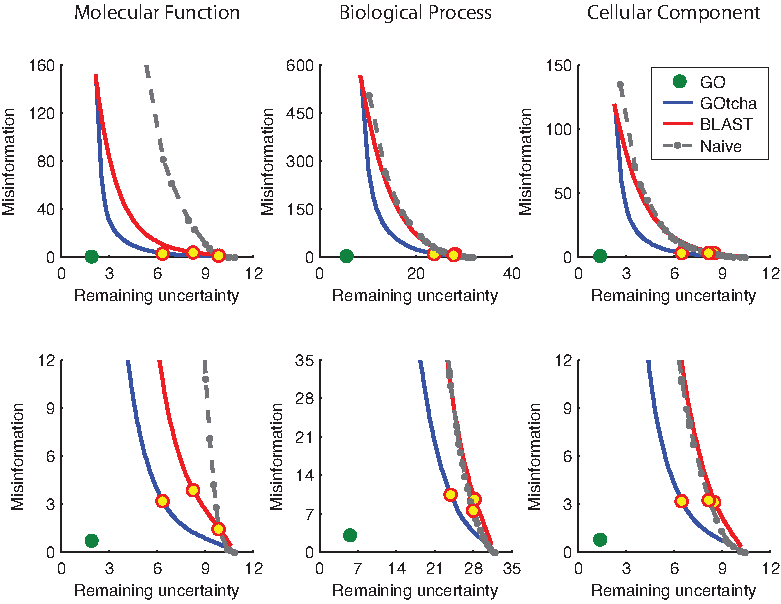
\includegraphics[width=.85\linewidth]{Figures/rumi/S4}
\end{centering}
\caption[Detailed figures showing the $ru$ and $mi$ of baseline methods]{Figures showing the remaining uncertainty and misinformation of baseline methods with yellow dots denoting values at which each method obtains its $S_{2}$ value. For better interpretation of the values at which each method achieves its $S_{2}$ value the bottom row of figures show the same plots as the top row, but with adjusted y-axis limits. }
\label{fig:rumiS4}
\end{figure*}
%%%%%%%%%%%%%%%%%%%%%%
%%%%%%%%%%%%%%%%%%%%%%


The information-theoretic measures are shown in the last two columns of Figure \ref{fig:rumi4} and in Figure \ref{fig:rumiS4}. One useful property of ru-mi plots is that they explicitly illustrate how many bits of information are yet to be revealed about a protein (on average) as a function of misinformation that is introduced by over-prediction or misannotation. In all three categories, the amount of misinformation being introduced increases rapidly; quickly obtaining a rate that is twice the amount of expected information for an average protein. We believe these plots shed new light into how much information overload a researcher can be presented with by drawing predictions at a particular threshold. Looking from right to left in each plot, we observe an elbow in each of the curves (at about 3 bits for MFO and CCO and 12 bits for BPO; Figure \ref{fig:rumi4}) after which the remaining uncertainty barely decreases, while misinformation grows out of control.

 Figure \ref{fig:rumiS1} and Figure \ref{fid:rumiS2} show results when implementing the supplemental information theoretic metrics using all-pair and max-average methods of averaging, respectively. It is important to mention that in a direct application of Resnik's similarity function, we refer to it as \emph{Lord} in Figure \ref{fig:rumiS1} (all-pair averaging) and as \emph{Resnik} in Figure \ref{fid:rumiS2} (max-average method of averaging). This is because, to the best of our knowledge, in the context of comparing functional annotations of proteins the all-pair averaging was first proposed by \citet{Lord2003}.

%%%%%%%%%%%%%%%%%%%%%%
%%%%%%%%%%%%%%%%%%%%%%
\begin{figure*}[h!]
\begin{centering}
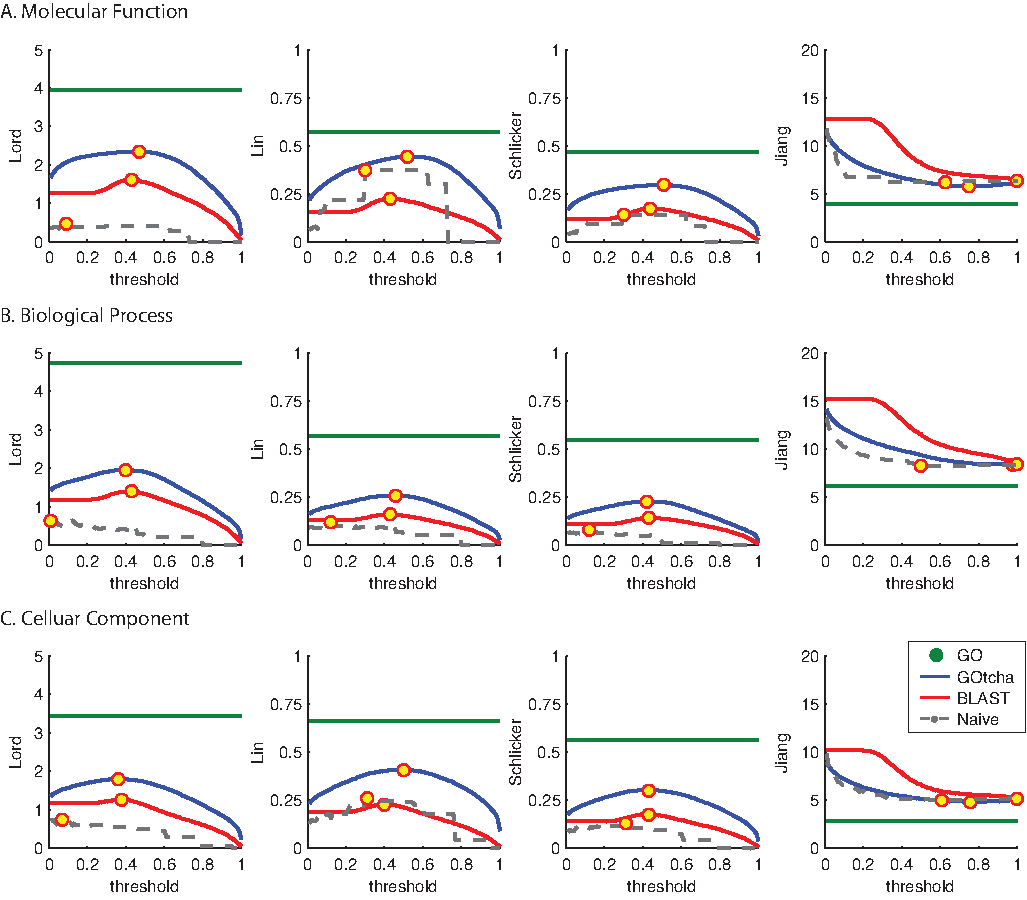
\includegraphics[width=\linewidth]{Figures/rumi/S1}
\par\end{centering}
\caption[Performance of information content-based metrics when using the all-pair method of averaging]{Two-dimensional evaluation plots of information content-based metric performances when using the all-pair method of averaging. Yellow dots denote the maximum similarity or, in the case of  \citet{Jiang1997}, the minimum distance, that each method obtains.}
\label{fig:rumiS1}
\end{figure*}
%%%%%%%%%%%%%%%%%%%%%%
%%%%%%%%%%%%%%%%%%%%%%

%%%%%%%%%%%%%%%%%%%%%%
%%%%%%%%%%%%%%%%%%%%%%
\begin{figure*}[h!]
\begin{centering}
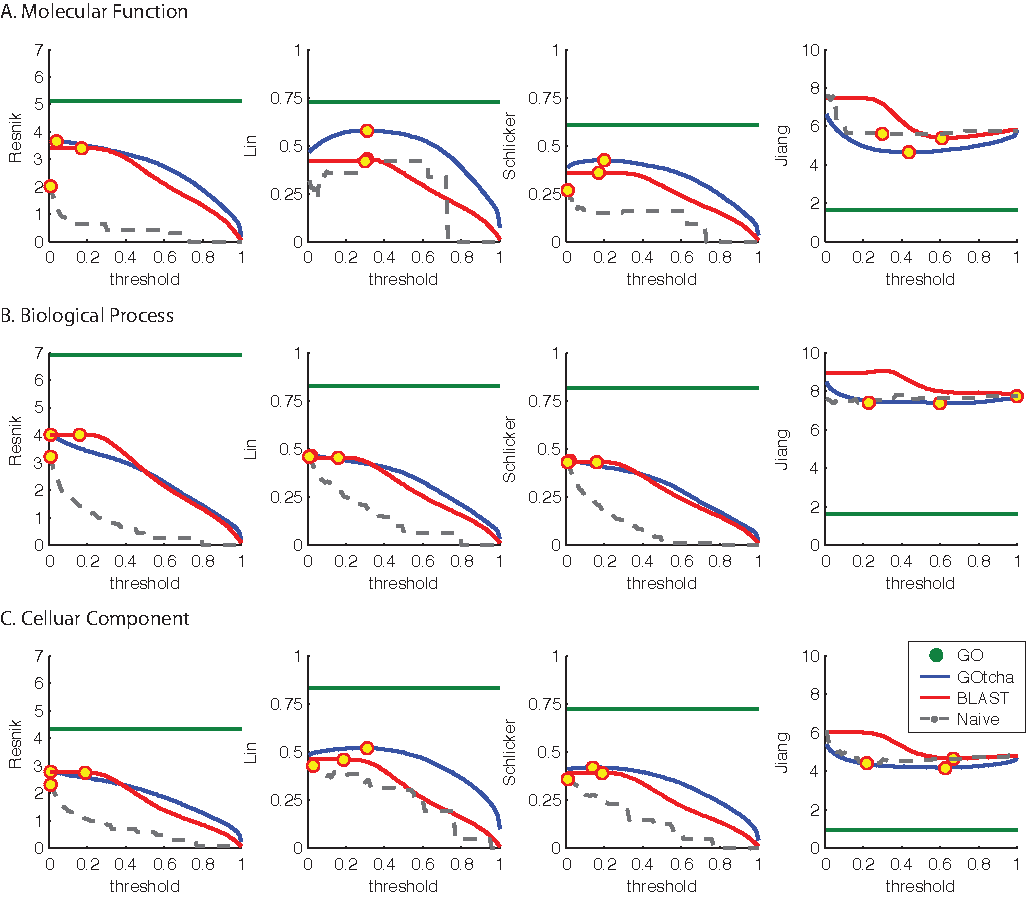
\includegraphics[width=\linewidth]{Figures/rumi/S2}
\par\end{centering}
\caption[Performance of iInformation content-based metric when using the max-average method of averaging]{Two-dimensional evaluation plots of information content-based metric performances when using the max-average method of averaging. Yellow dots denote the maximum similarity or, in the case of \citet{Jiang1997}, the minimum distance, that each method obtains.}
\label{fid:rumiS2}
\end{figure*}
%%%%%%%%%%%%%%%%%%%%%%
%%%%%%%%%%%%%%%%%%%%%%


In \Cref{fig:rumiS3} we contrast two different types of precision-recall curves. In the top row, we present the same results as in \Cref{fig:rumi3} of the main manuscript. In the bottom row, we use the max-averaging method for calculating precision-recall outlined by  \citet{Verspoor2006}. The methods provided similar results although the max-average formulation had generally larger values of $F_{\max}$ than the standard formulation of precision and recall (as defined in the main manuscript). However, these larger values of $F_{\max}$ occurred at lower decision thresholds.

%%%%%%%%%%%%%%%%%%%%%%
%%%%%%%%%%%%%%%%%%%%%%
\begin{figure*}[h!]
\begin{centering}
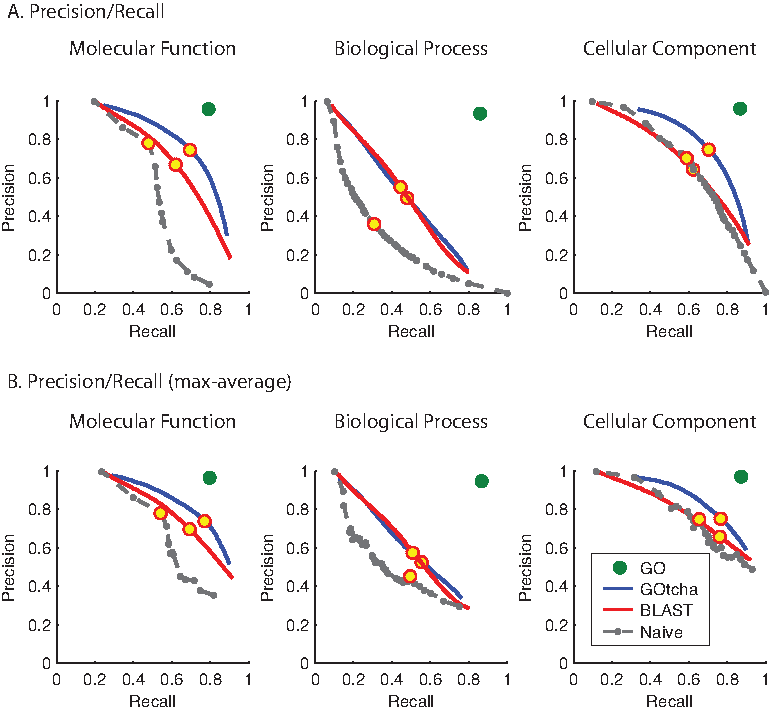
\includegraphics[width=.85\linewidth]{Figures/rumi/S3}
\par\end{centering}
\caption[Comparison of different methods of calculating precision and recall]{Plots showing results using the standard method of calculating precision and recall (top row) compared to using the max-average method of calculating precision and recall as detailed by \citet{Verspoor2006} (bottom row). Yellow dots denote the values of precision and recall at which each method obtains its $F_{\max}$ value. }
\label{fig:rumiS3}
\end{figure*}
%%%%%%%%%%%%%%%%%%%%%%
%%%%%%%%%%%%%%%%%%%%%%


%%%%%%%%%%%%%%%%%%%%%%
%%%%%%%%%%%%%%%%%%%%%%
\subsection{Comparisons of single statistics}
%%%%%%%%%%%%%%%%%%%%%%
%%%%%%%%%%%%%%%%%%%%%%

Here we analyze the ability of single measures to rank predictors and lead to useful evaluation insights. We compare the performance of semantic distance to several other methods that calculate either topological or semantic similarities. For each evaluation method, the decision threshold was varied for each of the prediction methods and the threshold providing the best performance was selected as optimal. We then analyze and discuss the performance of these metrics at those optimal thresholds.

We implemented the semantic similarity metrics of \cite{Resnik1995}, \cite{Jiang1997}, \cite{Lin1998}, and \cite{Schlicker2006}, as detailed in Section \ref{sec:rumisupmethods}. Because each of these measures is only defined for a single pair of terms in the ontology, scores between two protein annotation graphs (true graph $T$ vs. predicted graph $P$) we implemented both all pair averaging (\Cref{tab:rumi1_1,tab:rumi1_2}) and max-averaging (\Cref{tab:rumiS1}) for these metrics as detailed in Section \ref{sec:averaging}. We note that the all-pair averaging using Resnik's term similarity was implemented by \citet{Lord2003} in the context of GO annotations. In addition to these semantic measures, we also implemented the Jaccard similarity coefficient between the sets of vertices in the two annotation graphs (Section \ref{sec:rumiAddTop}). For precision/recall curves and ru-mi curves, we used $F_{\max}$ and $S_{2}$ measures as single values to obtain optimal thresholds.

Tables \ref{tab:rumi1_1}, \ref{tab:rumi1_1}, and \ref{tab:rumiS1} show the maximum similarity, or minimum distance in the case of Jiang and Conrath's and semantic distance, that each metric obtained for each of our classification models. In addition to reporting the maximum similarity we also report the decision threshold at which that value was obtained along with the associated level of remaining uncertainty and misinformation at that threshold. 

Considering \Cref{tab:rumi1_1,tab:rumi1_2} the first interesting observation is that all metrics, aside from that of Jiang and Conrath, obtain optimal thresholds that result in relatively similar levels of remaining uncertainty and misinformation for the GOtcha model. However, all metrics, aside from semantic distance and Jiang and Conrath's distance seem to favor extremely high levels of misinformation at the reported decision thresholds for the BLAST model. For MFO and CCO the semantic similarity measures of Lord \emph{et al.}, Lin and Sclicker \emph{et al.} report misinformation levels that are more than twice the information content of the average protein in that ontology for the BLAST model. In BPO those are even more extreme. We believe this is a direct consequence of the pairwise term averaging applied in these methods.

In Table \ref{tab:rumiS1}, we provide results analogous to those from Table \ref{tab:rumi1_1}, but using max-average method instead of all-pair averaging. We generally observe similar trends as before, but note that the values of BLAST thresholds used for functional transfer are even lower than when all-pair averaging was used (except for the measure by \citealt{Jiang1997}, where max-average method seems to be beneficial). 

%%%%%%%%%%%%%%%%%%%%%%
%%%%%%%%%%%%%%%%%%%%%%
\begin{table*}[t]
\caption[Performance evaluation of common information-theoretic metrics]{Performance evaluation of common information-theoretic metrics. For each measure, the decision threshold was varied across the entire range of predictions to obtain the maximum or minimum value (shown in column 1). The threshold at which each method reached the best value is shown in column 2. Columns 3 and 4 show the remaining uncertainty ($ru$) and misinformation ($mi$) calculated according to the Bayesian network. Each semantic similarity metric was calculated according to the relative frequencies of observing each term in the database. 
\label{tab:rumi1_1}}
\resizebox{\columnwidth}{!}
{\begin{tabular}{c|cccc|cccc|cccc}

\multicolumn{1}{l}{\hphantom} &\multicolumn{4}{c}{\bf Molecular Function } & \multicolumn{4}{c}{\bf Biological Process} &  \multicolumn{4}{c}{\bf Cellular Component } \\

\bf Lord & Max & Threshold & ru & mi & Max & Threshold & ru & mi & Max & Threshold & ru & mi\\
\hline
\multicolumn{1}{l|}{GOtcha}& 2.34 & 0.47 & 6.34 & 3.20 & 1.95 & 0.40 & 23.36 & 11.90 & 1.80 & 0.36 & 5.88 & 4.58 \\
\multicolumn{1}{l|}{BLAST}& 1.61 & 0.43 & 4.69 & 27.90 & 1.40 & 0.43 & 16.73 & 139.57 & 1.27 & 0.38 & 4.42 & 37.24 \\
\multicolumn{1}{l|}{Naive}& 0.46 & 0.09 & 9.56 & 4.23 & 0.63 & 0.01 & 10.35 & 504.88 & 0.75 & 0.07 & 5.81 & 16.34 \\


\multicolumn{1}{l}{\hphantom} & & & &\multicolumn{1}{c}{\hphantom} & & & & \multicolumn{1}{c}{\hphantom} & & & &\\

\bf Lin & Max & Threshold & ru & mi & Max & Threshold & ru & mi & Max & Threshold & ru & mi\\
\hline
\multicolumn{1}{l|}{GOtcha}& 0.44 & 0.52 & 6.67 & 2.67 & 0.26 & 0.46 & 24.43 & 9.40 & 0.41 & 0.50 & 6.71 & 2.76 \\
\multicolumn{1}{l|}{BLAST}& 0.22 & 0.43 & 4.69 & 27.90 & 0.16 & 0.43 & 16.73 & 139.57 & 0.23 & 0.40 & 4.78 & 30.45 \\
\multicolumn{1}{l|}{Naive}& 0.37 & 0.30 & 10.39 & 0.21 & 0.12 & 0.12 & 24.92 & 23.14 & 0.26 & 0.31 & 8.98 & 1.32 \\

\multicolumn{1}{l}{\hphantom} & & & &\multicolumn{1}{c}{\hphantom} & & & & \multicolumn{1}{c}{\hphantom} & & & &\\
%\hline
%\rowcolor{LightBlue}
\bf Schlicker & Max & Threshold & ru & mi & Max & Threshold & ru & mi & Max & Threshold & ru & mi\\
\hline
\multicolumn{1}{l|}{GOtcha}& 0.29 & 0.51 & 6.60 & 2.76 & 0.23 & 0.42 & 23.73 & 10.99 & 0.30 & 0.43 & 6.31 & 3.56 \\
\multicolumn{1}{l|}{BLAST}& 0.17 & 0.44 & 4.83 & 25.39 & 0.14 & 0.43 & 16.73 & 139.57 & 0.18 & 0.43 & 5.26 & 23.26 \\
\multicolumn{1}{l|}{Naive}& 0.14 & 0.30 & 10.39 & 0.21 & 0.08 & 0.12 & 24.92 & 23.14 & 0.13 & 0.31 & 8.98 & 1.32 \\

\multicolumn{1}{l}{\hphantom} & & & &\multicolumn{1}{c}{\hphantom} & & & & \multicolumn{1}{c}{\hphantom} & & & &\\

\bf Jiang & Min & Threshold & ru & mi & Min & Threshold & ru & mi & Min & Threshold & ru & mi\\
\hline
\multicolumn{1}{l|}{GOtcha}& 5.74 & 0.75 & 8.20 & 1.27 & 8.38 & 0.98 & 30.88 & 1.22 & 4.83 & 0.76 & 8.21 & 1.19 \\
\multicolumn{1}{l|}{BLAST}& 6.34 & 1.00 & 10.62 & 0.43 & 8.39 & 1.00 & 31.31 & 1.40 & 5.20 & 1.00 & 10.16 & 0.35 \\
\multicolumn{1}{l|}{Naive}& 6.19 & 0.63 & 10.53 & 0.13 & 8.24 & 0.50 & 31.75 & 0.07 & 5.01 & 0.61 & 10.13 & 0.08 \\


%\multicolumn{1}{l}{\hphantom} & & & &\multicolumn{1}{c}{\hphantom} & & & & \multicolumn{1}{c}{\hphantom} & & & &\\
%
%\bf Jaccard & Max & Threshold & ru & mi & Max & Threshold & ru & mi & Max & Threshold & ru & mi\\
%\hline
%\multicolumn{1}{l|}{GOtcha}& 0.57 & 0.46 & 6.29 & 3.32 & 0.31 & 0.34 & 22.24 & 15.24 & 0.56 & 0.43 & 6.31 & 3.56 \\
%\multicolumn{1}{l|}{BLAST}& 0.37 & 0.50 & 5.74 & 14.72 & 0.19 & 0.50 & 19.68 & 76.98 & 0.34 & 0.43 & 5.26 & 23.26 \\
%\multicolumn{1}{l|}{Naive}& 0.46 & 0.30 & 10.39 & 0.21 & 0.17 & 0.19 & 27.53 & 9.22 & 0.47 & 0.31 & 8.98 & 1.32 \\
%
%
%\multicolumn{1}{l}{\hphantom} & & & &\multicolumn{1}{c}{\hphantom} & & & & \multicolumn{1}{c}{\hphantom} & & & &\\
%
%$\mathbf{ F_{max} }$ & Max & Threshold & ru & mi & Max & Threshold & ru & mi & Max & Threshold & ru & mi\\
%\hline
%\multicolumn{1}{l|}{GOtcha}& 0.72 & 0.43 & 6.12 & 3.68 & 0.49 & 0.32 & 21.84 & 16.69 & 0.73 & 0.43 & 6.31 & 3.56 \\
%\multicolumn{1}{l|}{BLAST}& 0.64 & 0.48 & 5.42 & 17.89 & 0.49 & 0.50 & 19.68 & 76.98 & 0.63 & 0.45 & 5.57 & 19.42 \\
%\multicolumn{1}{l|}{Naive}& 0.60 & 0.29 & 9.87 & 1.44 & 0.33 & 0.19 & 27.53 & 9.22 & 0.64 & 0.33 & 9.22 & 0.80 \\
%
%
%\multicolumn{1}{l}{\hphantom} & & & &\multicolumn{1}{c}{\hphantom} & & & & \multicolumn{1}{c}{\hphantom} & & & &\\
%
%$\mathbf{S_{2}}$  & Min & Threshold & ru & mi & Max & Threshold & ru & mi & Max & Threshold & ru & mi\\
%\hline
%\multicolumn{1}{l|}{GOtcha}& 7.11 & 0.47 & 6.34 & 3.20 & 26.14 & 0.43 & 23.91 & 10.56 & 7.23 & 0.46 & 6.48 & 3.21 \\
%\multicolumn{1}{l|}{BLAST}& 9.13 & 0.77 & 8.25 & 3.90 & 29.89 & 0.88 & 28.28 & 9.69 & 9.08 & 0.78 & 8.51 & 3.15 \\
%\multicolumn{1}{l|}{Naive}& 9.98 & 0.10 & 9.72 & 2.80 & 29.00 & 0.22 & 27.67 & 8.72 & 8.79 & 0.21 & 7.71 & 4.95 \\

%\end{tabular}}{Values marked in bold are interesting .  Might want to say more, but really probably don't need to here.}
\end{tabular}}{}
\end{table*}
%%%%%%%%%%%%%%%%%%%%%%
%%%%%%%%%%%%%%%%%%%%%%



\begin{table*}[t]
\caption[Performance evaluation of topological metrics and $S_{2}$]{Performance evaluation of topological metrics and $S_{2}$. For each measure, the decision threshold was varied across the entire range of predictions to obtain the maximum or minimum value (shown in column 1). The threshold at which each method reached the best value is shown in column 2. Columns 3 and 4 show the remaining uncertainty ($ru$) and misinformation ($mi$) calculated according to the Bayesian network. Each semantic similarity metric was calculated according to the relative frequencies of observing each term in the database. 
\label{tab:rumi1_2}}
\resizebox{\columnwidth}{!}
{\begin{tabular}{c|cccc|cccc|cccc}

\multicolumn{1}{l}{\hphantom} &\multicolumn{4}{c}{\bf Molecular Function } & \multicolumn{4}{c}{\bf Biological Process} &  \multicolumn{4}{c}{\bf Cellular Component } \\

\bf Jaccard & Max & Threshold & ru & mi & Max & Threshold & ru & mi & Max & Threshold & ru & mi\\
\hline
\multicolumn{1}{l|}{GOtcha}& 0.57 & 0.46 & 6.29 & 3.32 & 0.31 & 0.34 & 22.24 & 15.24 & 0.56 & 0.43 & 6.31 & 3.56 \\
\multicolumn{1}{l|}{BLAST}& 0.37 & 0.50 & 5.74 & 14.72 & 0.19 & 0.50 & 19.68 & 76.98 & 0.34 & 0.43 & 5.26 & 23.26 \\
\multicolumn{1}{l|}{Naive}& 0.46 & 0.30 & 10.39 & 0.21 & 0.17 & 0.19 & 27.53 & 9.22 & 0.47 & 0.31 & 8.98 & 1.32 \\


\multicolumn{1}{l}{\hphantom} & & & &\multicolumn{1}{c}{\hphantom} & & & & \multicolumn{1}{c}{\hphantom} & & & &\\

$\mathbf{ F_{max} }$ & Max & Threshold & ru & mi & Max & Threshold & ru & mi & Max & Threshold & ru & mi\\
\hline
\multicolumn{1}{l|}{GOtcha}& 0.72 & 0.43 & 6.12 & 3.68 & 0.49 & 0.32 & 21.84 & 16.69 & 0.73 & 0.43 & 6.31 & 3.56 \\
\multicolumn{1}{l|}{BLAST}& 0.64 & 0.48 & 5.42 & 17.89 & 0.49 & 0.50 & 19.68 & 76.98 & 0.63 & 0.45 & 5.57 & 19.42 \\
\multicolumn{1}{l|}{Naive}& 0.60 & 0.29 & 9.87 & 1.44 & 0.33 & 0.19 & 27.53 & 9.22 & 0.64 & 0.33 & 9.22 & 0.80 \\


\multicolumn{1}{l}{\hphantom} & & & &\multicolumn{1}{c}{\hphantom} & & & & \multicolumn{1}{c}{\hphantom} & & & &\\

$\mathbf{S_{2}}$  & Min & Threshold & ru & mi & Min & Threshold & ru & mi & Min & Threshold & ru & mi\\
\hline
\multicolumn{1}{l|}{GOtcha}& 7.11 & 0.47 & 6.34 & 3.20 & 26.14 & 0.43 & 23.91 & 10.56 & 7.23 & 0.46 & 6.48 & 3.21 \\
\multicolumn{1}{l|}{BLAST}& 9.13 & 0.77 & 8.25 & 3.90 & 29.89 & 0.88 & 28.28 & 9.69 & 9.08 & 0.78 & 8.51 & 3.15 \\
\multicolumn{1}{l|}{Naive}& 9.98 & 0.10 & 9.72 & 2.80 & 29.00 & 0.22 & 27.67 & 8.72 & 8.79 & 0.21 & 7.71 & 4.95 \\

%\end{tabular}}{Values marked in bold are interesting .  Might want to say more, but really probably don't need to here.}
\end{tabular}}{}
\end{table*}
%%%%%%%%%%%%%%%%%%%%%%
%%%%%%%%%%%%%%%%%%%%%%




It is particularly interesting to analyze the optimal thresholds obtained for the BLAST model. These thresholds can be interpreted as the level of sequence identity above which each metric reports  functional transfer can be made. For example, because their optimal BLAST thresholds are relatively low, the levels of misinformation provided by the similarities of Lord \emph{et al.}, Lin, and Schlicker \emph{et al.} are rather large in both tables. $F_{\max}$ and Jaccard approaches also report low threshold values for all ontologies, while Jiang and Conrath's distance selects the optimal threshold at an overly restrictive 100\% sequence identity. We believe that the semantic distance $S_2$ provides more reasonable values for functional transfer, finding an optimal distance at 77\%, 88\% and 78\% for MFO, BPO, and CCO, respectively.

We believe that, generally, all-pair averaging provides better results regarding functional similarity than does max-average.  This is predominantly based on the even lower optimal thresholds obtained for the BLAST model in Table \ref{tab:rumiS1}.

%%%%%%%%%%%%%%%%%%%%%%
%%%%%%%%%%%%%%%%%%%%%%
\begin{table*}[h!]
\caption[Performance evaluation of metrics using max-averaging]{Performance of information-theoretic methods when calculating performance as the average of maximum similarity (or distance) between each true and predicted term as described in Section \ref{sec:averaging}. $F_{\max}$ values were calculated using precision and recall as detailed by  \citet{Verspoor2006}. The decision threshold was varied across the entire range of predictions to obtain the maximum or minimum value (shown in column 1) for each method. The threshold at which each method reached the best value is shown in column 2. Columns 3 and 4 show the remaining uncertainty and misinformation calculated according to the Bayesian network.
\label{tab:rumiS1}}
\resizebox{\columnwidth}{!}
{\begin{tabular}{c|cccc|cccc|cccc}

\multicolumn{1}{l}{\hphantom} &\multicolumn{4}{c}{\bf Molecular Function } & \multicolumn{4}{c}{\bf Biological Process} &  \multicolumn{4}{c}{\bf Cellular Component } \\


\bf Resnik & Max & Threshold & ru & mi & Max & Threshold & ru & mi & Max & Threshold & ru & mi\\
\hline
\multicolumn{1}{l|}{GOtcha}& 3.65 & 0.04 & 2.96 & 32.17 & 4.02 & 0.01 & 10.19 & 273.90 & 2.80 & 0.01 & 2.70 & 59.02 \\
\multicolumn{1}{l|}{BLAST}& 3.41 & 0.17 & 2.17 & 151.77 & 4.03 & 0.16 & 8.48 & 566.88 & 2.77 & 0.19 & 2.26 & 119.34 \\
\multicolumn{1}{l|}{Naive}& 2.02 & 0.01 & 5.07 & 177.91 & 3.22 & 0.01 & 10.35 & 504.88 & 2.32 & 0.01 & 2.65 & 135.04 \\


\multicolumn{1}{l}{\hphantom} & & & &\multicolumn{1}{c}{\hphantom} & & & & \multicolumn{1}{c}{\hphantom} & & & &\\

\bf Lin & Max & Threshold & ru & mi & Max & Threshold & ru & mi & Max & Threshold & ru & mi\\
\hline
\multicolumn{1}{l|}{GOtcha}& 0.58 & 0.31 & 5.32 & 5.86 & 0.46 & 0.02 & 11.10 & 192.89 & 0.52 & 0.31 & 5.55 & 5.58 \\
\multicolumn{1}{l|}{BLAST}& 0.43 & 0.31 & 2.90 & 90.72 & 0.45 & 0.16 & 8.48 & 566.88 & 0.46 & 0.19 & 2.26 & 119.34 \\
\multicolumn{1}{l|}{Naive}& 0.42 & 0.30 & 10.39 & 0.21 & 0.46 & 0.01 & 10.35 & 504.88 & 0.43 & 0.03 & 3.90 & 56.83 \\


\multicolumn{1}{l}{\hphantom} & & & &\multicolumn{1}{c}{\hphantom} & & & & \multicolumn{1}{c}{\hphantom} & & & &\\

\bf Jiang & Min & Threshold & ru & mi & Min & Threshold & ru & mi & Min & Threshold & ru & mi\\
\hline
\multicolumn{1}{l|}{GOtcha}& 4.65 & 0.44 & 6.18 & 3.56 & 7.39 & 0.60 & 26.65 & 5.30 & 4.19 & 0.63 & 7.45 & 1.80 \\
\multicolumn{1}{l|}{BLAST}& 5.38 & 0.61 & 6.97 & 7.58 & 7.75 & 1.00 & 31.31 & 1.40 & 4.67 & 0.67 & 7.84 & 5.13 \\
\multicolumn{1}{l|}{Naive}& 5.61 & 0.30 & 10.39 & 0.21 & 7.41 & 0.23 & 27.73 & 8.49 & 4.45 & 0.22 & 8.17 & 3.25 \\


\multicolumn{1}{l}{\hphantom} & & & &\multicolumn{1}{c}{\hphantom} & & & & \multicolumn{1}{c}{\hphantom} & & & &\\

\bf Schlicker & Max & Threshold & ru & mi & Max & Threshold & ru & mi & Max & Threshold & ru & mi\\
\hline
\multicolumn{1}{l|}{GOtcha}& 0.42 & 0.20 & 4.56 & 9.32 & 0.44 & 0.02 & 11.10 & 192.89 & 0.42 & 0.14 & 4.29 & 12.76 \\
\multicolumn{1}{l|}{BLAST}& 0.36 & 0.17 & 2.17 & 151.77 & 0.43 & 0.16 & 8.48 & 566.88 & 0.39 & 0.19 & 2.26 & 119.34 \\
\multicolumn{1}{l|}{Naive}& 0.27 & 0.01 & 5.07 & 177.91 & 0.43 & 0.01 & 10.35 & 504.88 & 0.36 & 0.01 & 2.65 & 135.04 \\

\multicolumn{1}{l}{\hphantom} & & & &\multicolumn{1}{c}{\hphantom} & & & & \multicolumn{1}{c}{\hphantom} & & & &\\

$\mathbf{ F_{max} }$ & Max & Threshold & ru & mi & Max & Threshold & ru & mi & Max & Threshold & ru & mi\\
\hline
\multicolumn{1}{l|}{GOtcha}& 0.76 & 0.33 & 5.45 & 5.41 & 0.54 & 0.23 & 19.79 & 26.04 & 0.76 & 0.31 & 5.55 & 5.58 \\
\multicolumn{1}{l|}{BLAST}& 0.70 & 0.44 & 4.83 & 25.39 & 0.54 & 0.46 & 18.06 & 108.73 & 0.71 & 0.37 & 4.23 & 41.17 \\
\multicolumn{1}{l|}{Naive}& 0.64 & 0.29 & 9.87 & 1.44 & 0.47 & 0.07 & 22.06 & 51.55 & 0.70 & 0.20 & 7.23 & 6.75 \\


\end{tabular}}{}
\end{table*}
%%%%%%%%%%%%%%%%%%%%%%
%%%%%%%%%%%%%%%%%%%%%%


%\vskip -0.5in

%\begin{table}
%\processtable{BLAST threshold that produces the optimal score for each of the metrics. BLAST score provides sequence identity above which the metrics favor transfer of function from each protein in the database to the target protein. 
%\label{Tab:02}}
%{\begin{tabular}{l|cccccc|c}

%\multicolumn{1}{l|}{\hphantom} & \bf Lord & \bf Lin & \bf Schlicker & \bf Jiang  & \bf Jaccard & $%\mathbf{ F_{max} }$ & $\mathbf{S_{2}}$ \\
%\hline
%\bf MFO & 0.43 & 0.43 & 0.44 & 1 & 0.5 & 0.48 & 0.77\\
%\bf BPO & 0.43 & 0.43 & 0.43 & 1 & 0.5 & 0.5 & 0.88\\
%\bf CCO  & 0.38 & 0.4 & 0.43 & 1 & 0.43 & 0.45 & 0.78\\

%\end{tabular}}{Values marked in bold are interesting .  Might want to say more, but really probably don't need to here.}
%\end{tabular}}{}
%\end{table}





%%%%%%%%%%%%%%%%%%%%%%
%%%%%%%%%%%%%%%%%%%%%%



\section{Discussion}

Here we introduce an information-theoretic framework for evaluating the performance of computational protein function prediction. We frame protein function prediction as a structured-output learning problem in which the output space is represented by consistent subgraphs of the GO graph. We argue that our approach directly addresses evaluation in cases where there are multiple true and predicted (leaf) terms associated with a protein by taking the structure of the ontology and the dependencies between terms induced by a hierarchical ontology into account. Our method also facilitates accounting for the high level of biased and incomplete experimental annotations of proteins by allowing for the weighting of proteins based on the information content of their annotations. Because we maintain an information-theoretic foundation, our approach is relatively immune to the potential dissociation between the depth of a term and its information content; a weakness of often-used topological metrics in this domain such as precision/recall or ROC based evaluation. At the same time, because we take a holistic approach to considering a protein's potentially large set of true or predicted functional associations we resolve many of the problems introduced by the practice of aggregating multiple pairwise similarity comparisons common to existing semantic similarity measures.

Although there is a long history \citep{Resnik1999} and a significant body of work in the literature regarding the use of semantic similarity measures \citep{Pesquita2009,Guzzi2012}, to the best of our knowledge all such metrics are based on single statistics and are unable to provide insight into the levels of remaining uncertainty and misinformation that every predictor is expected to balance. Therefore, the methods proposed in this work extend, modify, and formalize several useful information-theoretic metrics introduced over the past decades. In addition, both remaining uncertainty and misinformation have natural information-theoretic interpretations and can provide meaningful information to the users of computational tools. At the same time, the semantic distance based on these concepts facilitates not only the use of a single performance measure to evaluate and rank predictors, but can also be exploited as a loss function during training.

One limitation of the proposed approach is grounded in the assumption that a Bayesian network, structured according to the underlying ontology, will perfectly model the prior probability distribution of a target variable. An interesting anomaly with this approach is that the marginal probability, and subsequently the information content, of a single term (i.e. consistent graph with a single leaf term) calculated by considering the conditional probabilities between child and parent terms in the graph does not necessarily match the relative term frequency in the database. \emph{Ad hoc} solutions that maintain the term information content are possible but would result in sacrificed interpretability of the metric itself. One such solution can be obtained via a recursive definition 
\[
ia(v)=i(v)-\sum_{u\in\mathcal{P}(v)}ia(u) 
\]
where $i(v)$ is estimated directly from the database and $ia(root)=0$.

Finally, rationalizing between evaluation metrics is a difficult task. The literature presents several strategies where protein sequence similarity, protein-protein interactions or other data are used to assess whether a performance metric behaves according to expectations \citep{Guzzi2012}. In this work, we took a somewhat different approach and showed that the demonstrably biased protein function data can be shown to provide surprising results with well-understood prediction algorithms and conventional evaluation metrics. Thus, we believe that our experiments provide evidence of the usefulness of the new evaluation metric.


